%\pdfoutput=1
% \documentclass[12pt,a4paper,superscriptaddress,preprint,longbibliography]{revtex4-1}
\documentclass[20pt]{extarticle}
% http://www-math.mit.edu/~psh/amshelp/2.3/template.tex
\usepackage[dvips]{graphicx}

\usepackage{mathtools}

\usepackage{geometry}
	\geometry{
	left=3mm,
	right=3mm,
	top=3mm,
	bottom=9mm,
	includefoot,
	footskip=5mm
	}

\usepackage{amssymb,amsmath}

\renewcommand{\labelitemii}{$\blacktriangleright$}

\usepackage{bm}
\usepackage{color}
\usepackage{colortbl}
\usepackage{tikz}
\definecolor{stayc}{RGB}{144,238,100}
\definecolor{shiftc}{RGB}{240,160,70}
\definecolor{threshc}{RGB}{30,40,230}

\usepackage{esvect}

\usepackage{supertabular}
\usepackage{multirow}
\usepackage{bigstrut}

\usepackage{ulem}
\newcommand{\del}[1]{\textcolor{red}{\sout{#1}}}
\newcommand{\ms}[1]{\textcolor{orange}{\bf [Michiko: #1]}}
\newcommand{\add}[1]{\textcolor{blue}{#1}}
\newcommand{\addd}[1]{\textcolor{orange}{#1}}
\newcommand{\naoki}[1]{\textcolor{green}{\bf [Naoki: #1]}}
\newcommand{\tw}[1]{\textcolor{cyan}{\bf [Takamitsu: #1]}}

\usepackage[hidelinks]{hyperref}
\newcommand{\hrefc}[2]{\href{#1}{\textcolor{blue}{#2}}}

\newcommand{\topdir}{../../..}

% Page number: bottom right, small font, on every page (incl. title page).
\usepackage{fancyhdr}
\pagestyle{fancy}
\fancyhf{}
\renewcommand{\headrulewidth}{0pt}
\renewcommand{\footrulewidth}{0pt}
\fancyfoot[R]{\footnotesize\thepage}
\fancypagestyle{plain}{%
	\fancyhf{}%
	\renewcommand{\headrulewidth}{0pt}%
	\renewcommand{\footrulewidth}{0pt}%
	\fancyfoot[R]{\footnotesize\thepage}%
}

\sloppy

% A compact 2x2 payoff matrix
\newcommand{\pdmatrix}[4]{%
\begin{center}
\begin{tabular}{|c||c|c|}
\hline
 & C & D \\
\hline\hline
C & #1 & #2 \\
\hline
D & #3 & #4 \\
\hline
\end{tabular}
\end{center}
}

\begin{document}

\title{MATH 463 Mathematical Biology\\
lecture notes\\
11. Evolutionary game theory}
\date{\today}
\author{Naoki Masuda}

\maketitle

\subsection*{Game theory: what and why?}

\begin{itemize}
%
\item Think why global warming is (probably) happening and difficult to handle.
%
\item \underline{Game theory}: mathematical modeling of decision making when agents influence each other. Represent benefit to each agent as a \emph{payoff} function.
	\begin{itemize}
	\item Book \hrefc{https://en.wikipedia.org/wiki/Theory_of_Games_and_Economic_Behavior}{``Theory of Games and Economic Behavior''} by John Von Neumann and Oskar Morgenstern (1944).
	\item Nash equilibrium by John Nash (Did you watch a 2001 film \hrefc{https://en.wikipedia.org/wiki/A_Beautiful_Mind_(film)}{``A Beautiful Mind''}?).
	\item 15 game theorists got Nobel Prize in Economics.
	\item A most recent one is \hrefc{https://en.wikipedia.org/wiki/Paul_Milgrom}{Paul Milgrom}, Stanford Prof, who did B.A. in Mathematics here!
	\item Not just for economics students!
	\end{itemize}
%
\item \underline{Evolutionary game theory}: When the agents are not rational decision makers, strategies that earn high payoffs spread by natural selection (or imitation, social learning).
	\begin{itemize}
	\item Originally, \hrefc{https://doi.org/10.1038/246015a0}{Maynard Smith \& Price, Logic of animal conflict, Nature (1973)} in mathematical biology.
	\item Also \hrefc{https://doi.org/10.1017/CBO9780511806292}{a famous book by Maynard Smith (1982)}.
	\item Used to model animal conflict, foraging, sex ratios, signaling, host--parasite coevolution, microbial cooperation, etc.
	\end{itemize}
\end{itemize}

\subsection*{Prisoner's dilemma (classical game theory yet)}

\pdmatrix{R}{S}{T}{P}
\begin{itemize}
\item R: reward,
\item T: temptation (to defect),
\item S: sucker ('s payoff),
\item P: punishment (for defecting).
\end{itemize}
or famously
\pdmatrix{3}{0}{5}{1}
or, in the original story of two suspects interrogated separately (years in prison):
\begin{center}
\renewcommand{\arraystretch}{1.4}
\begin{tabular}{|c||c|c|}
\hline
 & partner stays silent & partner betrays \\
\hline\hline
you stay silent & \cellcolor{stayc!50}1, 1 & \cellcolor{black!10}10, 0 \\
\hline
you betray & \cellcolor{black!10}0, 10 & \cellcolor{shiftc!60}5, 5 \\
\hline
\end{tabular}
\end{center}
Whatever the partner does, betraying shortens your own sentence, but both would be better off staying silent.

\subsubsection*{Assumptions}

\begin{itemize}
\item Each player ($=$ agent) has two actions/strategies, cooperate (C) or defect (D).
\item This is a two-person, symmetric game.
\item The numbers in the matrix represent what the \emph{row} player gets.
\item $T>R>P>S$ assumed. Different inequalities lead to (often important) other types of game.
	\begin{itemize}
	\item Chicken game (also called snowdrift game and hawk--dove game) if $T>R>S>P$.
	\end{itemize}
\end{itemize}

\subsubsection*{Observations}

\begin{itemize}
\item \textbf{Questions:}
	\begin{itemize}
	\item If the opponent player cooperates, should I cooperate or defect?
	\item If the opponent player defects, should I cooperate or defect?
	\end{itemize}
\item No matter what the other player does, it is more lucrative for each player to defect.
\item If both players defect, they both get $P$.
\item However, if both players cooperate, they both get $R$ ($>P$).
\end{itemize}

\subsection*{Nash equilibrium}

\begin{itemize}
\item \underline{Nash equilibrium}: a situation where no player can improve their payoff by unilaterally changing their strategy, given the strategy chosen by the other player.
\item Each player's strategy is an optimal response to the strategy of the other.
\item \textbf{Q:} What is the Nash equilibrium of the prisoner's dilemma game?
\item Formally, in a symmetric two-player game with payoff matrix $A$ (so that $A_{ij} = u(s_i, s_j)$ is the payoff to a player who plays $s_i$ against an opponent who plays $s_j$), strategy $x$ is Nash if
\[ u(x,x) \ge u(y,x) \quad \text{for every strategy } y. \]
A \emph{strict} Nash equilibrium replaces $\ge$ by $>$ for all $y \neq x$.
\item \textbf{Q:} Is the Nash equilibrium of the prisoner's dilemma game strict Nash or non-strict Nash?
\end{itemize}

\subsection*{Why \emph{evolutionary} game theory?}

This is a math bio course, not an economics game theory course!

\begin{itemize}
\item Classical game theory assumes players reason about each other and pick best responses. In biology, however,
	\begin{itemize}
	\item Strategies are often genetically hard-wired (e.g., body size, aggressiveness, mating type, cell type).
	\item Fitter organisms leave more offspring, so successful strategies become more common over generations (i.e., selection).
		\begin{itemize}
		\item \textbf{Q:} Who said it?
		\end{itemize}
	\item Fitness ($\approx$ payoff) of one organism depends on what others do. E.g.,
		\begin{itemize}
		\item Large beetles do well only because most are small.
		\item Toxin-producing bacteria do well only because there are sensitive bacteria to kill.
		\end{itemize}
	\end{itemize}
\end{itemize}

\subsection*{Body-size game}

\begin{itemize}
\item A species of beetle competes for food.
\item A mutation occurs that increases body size.
\item Large beetles claim more of the food but spend more energy on metabolism.
\item Payoffs, adapted from \hrefc{https://www.cs.cornell.edu/home/kleinber/networks-book/networks-book.pdf}{Easley \& Kleinberg, Networks, Crowds, and Markets, Ch.~7}:
\begin{center}
\begin{tabular}{|c||c|c|}
\hline
 & Small & Large \\
\hline\hline
Small & $5,\,5$ & $1,\,8$ \\
\hline
Large & $8,\,1$ & $3,\,3$ \\
\hline
\end{tabular}
\end{center}

\item Notice the structure: $T>R>P>S$ ($8>5>3>1$). This is a prisoner's dilemma.
	\begin{itemize}
	\item Yet another example: arms race in athletes for performance-enhancing drugs.
	\end{itemize}
\item But the question we ask is different from classical game theory.
	\begin{itemize}
	\item Beetles are not deciding their body size. Each is genetically hard-wired.
	\item So, we cannot ask ``what is each beetle's best response?''. Instead we ask:
		\begin{itemize}
		\item If a population is mostly small, can a few large mutants invade?
		\item If a population is mostly large, can a few small mutants invade?
		\end{itemize}
	\end{itemize}
\item Other empirical examples of biological prisoner's dilemmas:
	\begin{itemize}
	\item Tree height: tall trees over-shade short neighbors but bear a metabolic cost.
%	\item Virus replication: phage $\Phi 6$ vs.\ its defector mutant $\Phi H2$.
% [Need to verify this example.]
	\item Cancer: covered later.
	\end{itemize}
\end{itemize}

\subsection*{Evolutionarily stable strategy (ESS)}

\begin{itemize}
%
\item Nash equilibrium answers: ``Is this strategy a best response to itself?''
%
\item In biology, we want to answer:
\begin{quote}
If almost everyone in a large population uses strategy $x$, and a small number of mutants enter playing a different strategy $y$, will the mutants be wiped out by selection?
\end{quote}
%
\item Nash is not enough:
	\begin{itemize}
	\item Many Nash equilibria are only \emph{weakly} stable: an alternative best response $y$ does just as well against $x$, so a tiny invading group of $y$-players is not eliminated; it can increase in frequency and even take over.
	\item Recap: Nash iff $u(x,x) \ge u(y,x)$ for every strategy $y$.
	\ \\
	\ \\
	\ \\
	\ \\
	\ \\
	\end{itemize}
%
\item ESS (evolutionary stable strategy): a refinement of Nash that captures evolutionary robustness to invasion by rare mutants.
%
\end{itemize}

\begin{itemize}
\item A strategy $s$ is evolutionarily stable if there is some small $\varepsilon_0 > 0$ such that, whenever any other strategy $s'$ invades $s$ at any level $\varepsilon < \varepsilon_0$,
\[ \text{fitness of an $s$-player} \;>\; \text{fitness of a $s'$-player}. \]
	\begin{itemize}
	\item $>$ cannot be replaced by $\ge$
	\end{itemize}
\end{itemize}

\subsubsection*{Definition of ESS}

\begin{itemize}
\item $S = \{ s_1, \ldots, s_N \}$ is the space of pure strategies.
\item $A_{ij}=u(s_i,s_j)$ is the payoff matrix.
\item $x = \begin{pmatrix} x_1\\ \vdots \\ x_N \end{pmatrix}, y = \begin{pmatrix} y_1\\ \vdots \\ y_N \end{pmatrix}$: mixed strategies (probability distributions over $S$).
\item $u(x,y) = x^{\top} A\, y = \sum_{i=1}^N \sum_{j=1}^N x_i A_{ij} y_j = \text{ payoff to } x$.
	\begin{itemize}
	\item \textbf{Q:} Does this definition work? Check with $A =$ \pdmatrix{3}{0}{5}{1}.
	\item What is $N$?
	\item What is vector $x$ if $x$ corresponds to cooperation?
	\item Compute $x^{\top} A x$. What does this value mean?
	\item What is vector $y$ if $y$ corresponds to defection?
	\item Compute $x^{\top} A y$. What does this value mean?
	\ \\
	\ \\
	\ \\
	\end{itemize}
\item $u$ is bilinear:
\[ u(\alpha x + (1-\alpha)y,\, z) = \alpha\, u(x,z) + (1-\alpha)\, u(y,z), \]
\[ u(x,\, \alpha y + (1-\alpha) z) = \alpha\, u(x,y) + (1-\alpha)\, u(x,z). \]
\end{itemize}

\begin{itemize}
\item \textbf{Definition.} A (mixed) strategy $x$ is \emph{evolutionarily stable} if, for every $y \neq x$, there exists $\varepsilon_y > 0$ such that
\[ u\bigl(x,\, (1-\varepsilon)x + \varepsilon y\bigr) > u\bigl(y,\, (1-\varepsilon)x + \varepsilon y\bigr) \]
for every $\varepsilon \in (0, \varepsilon_y]$.
%
\item Then, mutants are eliminated by selection.
	\begin{itemize}
	\item \textbf{Q:} Which is the mutant, $x$ or $y$?
	\item Intuition is ...
	\ \\
	\ \\
	\ \\
	\ \\
	\end{itemize}
%
\end{itemize}

An alternative (and more useful) characterization (definition) is:
\begin{itemize}
\item $x$ is an ESS if and only if for every $y \neq x$,
	\begin{enumerate}
	\item $u(x,x) \ge u(y,x)$ \qquad (Nash condition), and
	\item if $u(x,x) = u(y,x)$, then $u(x,y) > u(y,y)$.
	\end{enumerate}
%
% \item \emph{Proof.} Define $F(\varepsilon,y) = u\bigl(x,(1-\varepsilon)x+\varepsilon y\bigr) - u\bigl(y,(1-\varepsilon)x+\varepsilon y\bigr)$. Using bilinearity,
% \[ F(\varepsilon,y) = u(x-y,\, x + \varepsilon(y-x)) = u(x-y,x) + \varepsilon\, u(x-y, y-x). \]
% ESS demands $F(\varepsilon,y) > 0$ for all small $\varepsilon > 0$. The first term $u(x-y,x) = u(x,x) - u(y,x)$ must be $\ge 0$; if it equals $0$, then the sign is determined by the second term, $u(x-y,y-x) = u(x,y) - u(y,y) - u(x,x) + u(y,x) = u(x,y) - u(y,y) > 0$.
%
\end{itemize}

\textbf{Another fact:} 
\[ \text{strict Nash} \;\subsetneq\; \text{ESS} \;\subsetneq\; \text{Nash}. \]

\subsubsection*{ESS in the body-size game}

The beetle payoffs again:
\begin{center}
\begin{tabular}{|c||c|c|}
\hline
 & Small & Large \\
\hline\hline
Small & $5,\,5$ & $1,\,8$ \\
\hline
Large & $8,\,1$ & $3,\,3$ \\
\hline
\end{tabular}
\end{center}

\noindent\textbf{Is Small an ESS?} \\
Condition to check: $u\bigl(x,\, (1-\varepsilon)x + \varepsilon y\bigr) > u\bigl(y,\, (1-\varepsilon)x + \varepsilon y\bigr)$\\
Suppose a fraction $\varepsilon$ of the population is Large.
\begin{itemize}
\item A Small beetle meets Small with prob.\ $1-\varepsilon$ (payoff 5) and Large with prob.\ $\varepsilon$ (payoff 1):
\[ \text{fitness(Small)} = 5(1-\varepsilon) + 1\cdot\varepsilon = 5 - 4\varepsilon. \]
\item A Large mutant meets Small with prob.\ $1-\varepsilon$ (payoff 8) and Large with prob.\ $\varepsilon$ (payoff 3):
\[ \text{fitness(Large)} = 8(1-\varepsilon) + 3\cdot\varepsilon = 8 - 5\varepsilon. \]
\item For all small $\varepsilon$ (in fact for $\varepsilon < 1$), fitness(Large) $>$ fitness(Small). \\
So, Small is NOT evolutionarily stable.
	\begin{itemize}
	\item You may know this without this calculation because Small not even Nash.
	\end{itemize}
\end{itemize}

\noindent\textbf{Is Large an ESS?} Now let $\varepsilon$ be the fraction of Small invaders.
\begin{itemize}
\item fitness(Large) $= 3(1-\varepsilon) + 8\varepsilon = 3 + 5\varepsilon$.
\item fitness(Small) $= 1(1-\varepsilon) + 5\varepsilon = 1 + 4\varepsilon$.
\item fitness(Large) $>$ fitness(Small) for all small $\varepsilon$. \\
So, Large IS evolutionarily stable.
\end{itemize}

\noindent\textbf{Reading.}
\begin{itemize}
\item In a population of small beetles, a rare large mutant wins almost every food fight and spreads.
\item In a population of large beetles, a rare small mutant loses almost every fight and dies out.
\end{itemize}

\subsection*{Hawk--dove game}

\begin{center}
\begin{tabular}{|c||c|c|}
\hline
 & H (Hawk) & D (Dove) \\
\hline\hline
H & $\bigl((V-c)/2,\,(V-c)/2\bigr)$ & $(V,\,0)$ \\
\hline
D & $(0,\,V)$ & $(V/2,\,V/2)$ \\
\hline
\end{tabular}
\end{center}

A textbook normalization is $V=2$, so

\begin{center}
\begin{tabular}{|c||c|c|}
\hline
 & H & D \\
\hline\hline
H & $(1-c,\,1-c)$ & $(2,\,0)$ \\
\hline
D & $(0,\,2)$ & $(1,\,1)$ \\
\hline
\end{tabular}
\end{center}

\begin{itemize}
\item Two animals contest a resource of value $V$ (food, territory, mate).
\item Hawk: escalate and fight. If both escalate, they injure each other; cost $c$ split between them.
\item Dove: display and retreat. Two doves share the resource peacefully.
\item Models the evolution of aggression: how aggressive should an organism be?
\end{itemize}

\subsubsection*{Two cases}

\begin{itemize}
\item Case 1: $c < 1$ (cheap fights, i.e., $V > c$).
	\begin{itemize}
	\item \textbf{Q:} Is H or D Nash?
	\end{itemize}
	\ \\
	\ \\
	\ \\
H strictly dominates D. The unique Nash and unique ESS is ``always Hawk.'' Every animal should be aggressive.
%
\item Case 2: $c > 1$ (costly fights, i.e., $V < c$).
	\begin{itemize}
	\item \textbf{Q:} Is H or D Nash?
	\end{itemize}
	\ \\
	\ \\
	\ \\
Neither pure strategy is Nash. There is a unique \emph{mixed} ESS:
\[ x^* = \left( \frac{V}{c},\; 1 - \frac{V}{c} \right) = \left( \frac{1}{c},\; 1 - \frac{1}{c} \right). \]
\item \textbf{Q:} Compute $x^*$ by setting $u(\text{H},x^*) = u(\text{D},x^*)$.
\item \textbf{Q:} Verify that $x^*$ satisfies the alternative ESS conditions.
\item Biological prediction: the fraction of aggressive individuals is determined by $V/c$, not by individual rationality. Empirically supported in many species (e.g., territorial contests).
\end{itemize}

\subsection*{Rock--scissors--paper}

We did it in mathematical ecology, but here as an evolutionary game.
\begin{center}
\begin{tabular}{|c||c|c|c|}
\hline
 & R & S & P \\
\hline\hline
R & $0,0$ & $1,-1$ & $-1,1$ \\
\hline
S & $-1,1$ & $0,0$ & $1,-1$ \\
\hline
P & $1,-1$ & $-1,1$ & $0,0$ \\
\hline
\end{tabular}
\end{center}

\begin{itemize}
\item Unique Nash equilibrium $s^* = \begin{pmatrix} 1/3 \\ 1/3 \\ 1/3 \end{pmatrix}$.
\item \textbf{Q:} Are ``corner'' equilibria Nash?
\item However: $s^*$ is not an ESS.
\item \textbf{Q:} Show this by exhibiting a mutant $y \neq s^*$ for which the ESS conditions fail. (This may be a difficult Q.)
\end{itemize}

\subsection*{From two players to a population}

\begin{itemize}
\item Real biological populations contain many players, not just two.
\item Two complementary approaches:
	\begin{itemize}
	\item Agent-based simulations:
		\begin{itemize}
		\item Many players, paired randomly or via a network.
		\item Necessarily a finite population.
		\item Each player updates by mimicking successful neighbors (social learning or reproduction).
		\item The update rule (how a player with payoff $f_i$ mimics another with payoff $f_j$) matters a lot.
		\end{itemize}
	\item ODE analysis:
		\begin{itemize}
		\item Track the fractions $x_1(t),\ldots,x_n(t)$ of each strategy in an infinite, well-mixed population.
		\item The gold standard is the replicator equation.
		\end{itemize}
	\end{itemize}
\end{itemize}

\begin{figure}[h]
\begin{center}
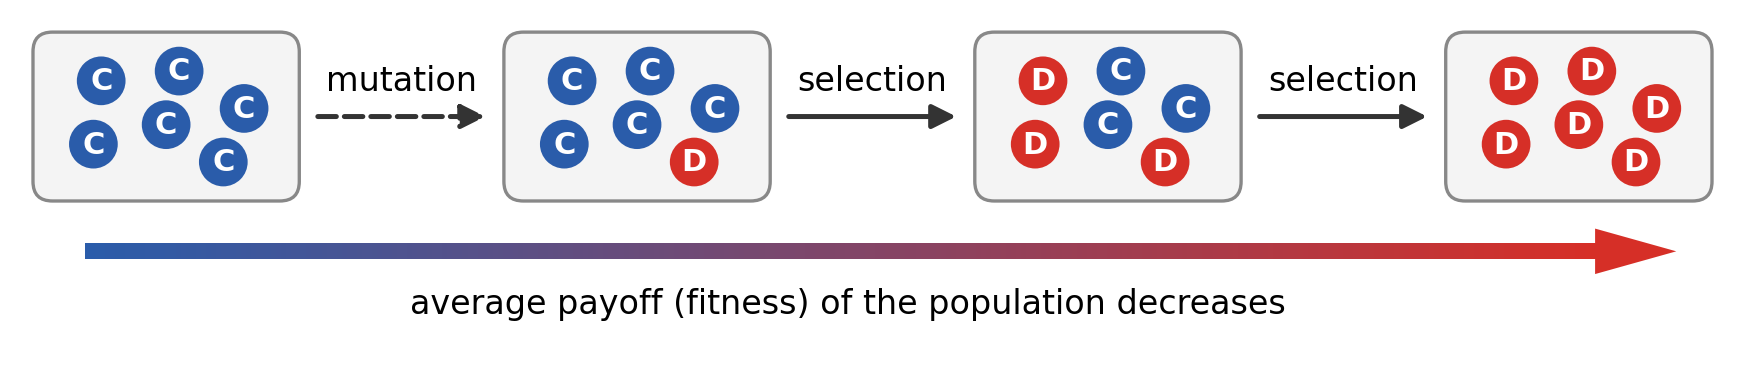
\includegraphics[width=0.85\textwidth]{figures/11_evolutionary-games/defection-takeover.png}
\caption{In a well-mixed population, defectors (D) take over cooperators (C). Redrawn after Fig.~1 of \hrefc{https://www.doi.org/10.1126/science.1133755}{Nowak, Science (2006)}.}
\end{center}
\end{figure}

\subsection*{Replicator equation}

\begin{itemize}
\item $p_i(t) = $ number of players using strategy $s_i$ at time $t$.
\item $p(t) = \sum_{i=1}^N p_i(t) = $ total population at time $t$.
\item $x_i(t) = p_i(t)/p(t)$
\item vector $x(t) = (x_1(t), \ldots, x_N(t))^{\top}$.
\item Average payoff in the population: $u(x,x) = \sum_{i=1}^N x_i\, u(s_i,x)$.
\item Per capita birth rate of strategy $s_i$: $\beta + u(s_i, x(t))$.
\item Death rate: $\delta$.
\item Hence
\[ \dot p_i = \left[\beta + u(s_i,x) - \delta\right] p_i, \]
\[ \dot p = \left[\beta + u(x,x) - \delta\right] p. \]
\item Differentiating $x_i = p_i / p$,
\[ \dot x_i = \frac{\dot p_i}{p} - \frac{p_i}{p^2}\, \dot p = \left[u(s_i,x) - u(x,x)\right] x_i. \]
\item The fraction of strategy $s_i$ grows if and only if it earns above-average payoff.
\item Even the second best strategy grows if it earns above-average payoff.
\end{itemize}

% \subsubsection*{Basic dynamical systems vocabulary}

% \begin{itemize}
% \item Let $F^t : \Theta \to \Theta$ be the flow of the ODE on the simplex $\Theta = \{x : x_i \ge 0,\ \sum_i x_i = 1\}$.
% \item \underline{Steady state}: $F^t(\theta) = \theta$ for all $t$ (equivalently, $\dot\theta = 0$).
% \item \underline{Stable steady state}: every neighborhood $U$ of $\theta$ contains a neighborhood $U_1$ such that $\theta_0 \in U_1 \Longrightarrow F^t(\theta_0) \in U$ for all $t \ge 0$.
% \item \underline{Asymptotically stable}: stable, and there exists a neighborhood $U$ with $\theta_0 \in U \Longrightarrow \lim_{t\to\infty} F^t(\theta_0) = \theta$.
% \end{itemize}

\subsection*{Replicator dynamics for the prisoner's dilemma}

\begin{itemize}
\item $x = $ fraction of cooperators,
\item $y = 1-x = $ fraction of defectors.
\item Payoffs:
\[
\begin{aligned}
f_{\text{C}} &= xR + yS,\\
f_{\text{D}} &= xT + yP,\\
\overline{f} &= x f_{\text{C}} + y f_{\text{D}}.
\end{aligned}
\]
\item Replicator equation:
\[
\begin{aligned}
\dot{x} &= x ( f_{\text{C}} - \overline{f} )
= x(1-x)\bigl[(xR+yS) - (xT+yP)\bigr]\\
&= x(1-x)\bigl[x(R-T) + y(S-P)\bigr],\\
\dot{y} &= -\,\dot x.
\end{aligned}
\]
\item One equation suffices because $y = 1-x$.
\item \textbf{Question:} Verify $\dot x + \dot y = 0$.
\item \textbf{Question:} With $T>R>P>S$, what happens? Recall

\pdmatrix{R}{S}{T}{P}

\item \textbf{Exercise:} Draw a phase portrait on $x \in [0,1]$. Identify the equilibria and their stability.
\item Conclusion: in a well-mixed population, cooperation goes extinct.
\end{itemize}

\subsubsection*{Replicator dynamics for the coordination game}

\begin{itemize}
\item Take $R>T$ and $P>S$, e.g.,

\pdmatrix{5}{0}{0}{3}

\item \textbf{Exercise:}
	\begin{enumerate}
	\item What do you expect to happen?
	\item Write the replicator equation in terms of $x$.
	\item Draw a phase portrait in $x$ and identify all equilibria and their stability.
	\item Which opinion / social dynamics model does this resemble?
	\end{enumerate}
\end{itemize}

\subsection*{Replicator dynamics for hawk--dove}

\begin{itemize}
\item $x = $ fraction of Hawks,
\item $1-x = $ fraction of Doves.
\item Set $V=2$, $c > 1$ (costly fights).
\begin{center}
\begin{tabular}{|c||c|c|}
\hline
 & H & D \\
\hline\hline
H & $1-c$ & $2$ \\
\hline
D & $0$ & $1$ \\
\hline
\end{tabular}
\end{center}

\item \textbf{Exercise:}
	\begin{enumerate}
	\item Write down $\dot x$.
	\item Find all interior and boundary equilibria.
	\item Show that the interior equilibrium
	%
	% $x^* = 1/c$
	%
	is asymptotically stable on $(0,1)$, consistent with the mixed ESS we found.
	\end{enumerate}
\end{itemize}

\subsection*{Replicator dynamics for rock--scissors--paper}

\begin{itemize}
\item $x = \begin{pmatrix} x_{\rm R} \\ x_{\rm S} \\ x_{\rm P} \end{pmatrix}$ lives on the ``2-simplex'' $x_{\rm R}+x_{\rm S}+x_{\rm P}=1$.
\item Using
\[
A = \begin{pmatrix} 0 & 1 & -1 \\ -1 & 0 & 1 \\ 1 & -1 & 0 \end{pmatrix}
\]
(rows and columns ordered R, S, P;\\
R beats S, S beats P, P beats R),\\
and noting that $x^{\top} A x = 0$ because $A$ is antisymmetric (\textbf{Q:} Verify this.), the replicator equation
\[
\dot x_i = x_i\left[(Ax)_i - x^{\top}Ax\right] 
\]
becomes
\[
\begin{aligned}
\dot x_{\rm R} &= x_{\rm R}(x_{\rm S} - x_{\rm P}),\\
\dot x_{\rm S} &= x_{\rm S}(x_{\rm P} - x_{\rm R}),\\
\dot x_{\rm P} &= x_{\rm P}(x_{\rm R} - x_{\rm S}).
\end{aligned}
\]
\item Same as Lotka--Volterra formalism.
\item The unique interior equilibrium is $(1/3,1/3,1/3)^{\top}$.
% \item Replicator dynamics for $n$ strategies is mathematically equivalent to Lotka--Volterra equations for $n-1$ species (a classical result of Hofbauer), so this \emph{is} a Lotka--Volterra system in disguise; the very same ODE arises from a well-mixed interacting-particle (``cyclic Lotka--Volterra'') model of cyclic competition. (See \hrefc{https://www.hup.harvard.edu/books/9780674023383}{Nowak, \emph{Evolutionary Dynamics}, Harvard Univ.\ Press (2006)} and \hrefc{https://doi.org/10.1017/CBO9781139173179}{Hofbauer and Sigmund, \emph{Evolutionary Games and Population Dynamics}, Cambridge Univ.\ Press (1998)}.)
\end{itemize}

\begin{figure}[h]
\begin{center}
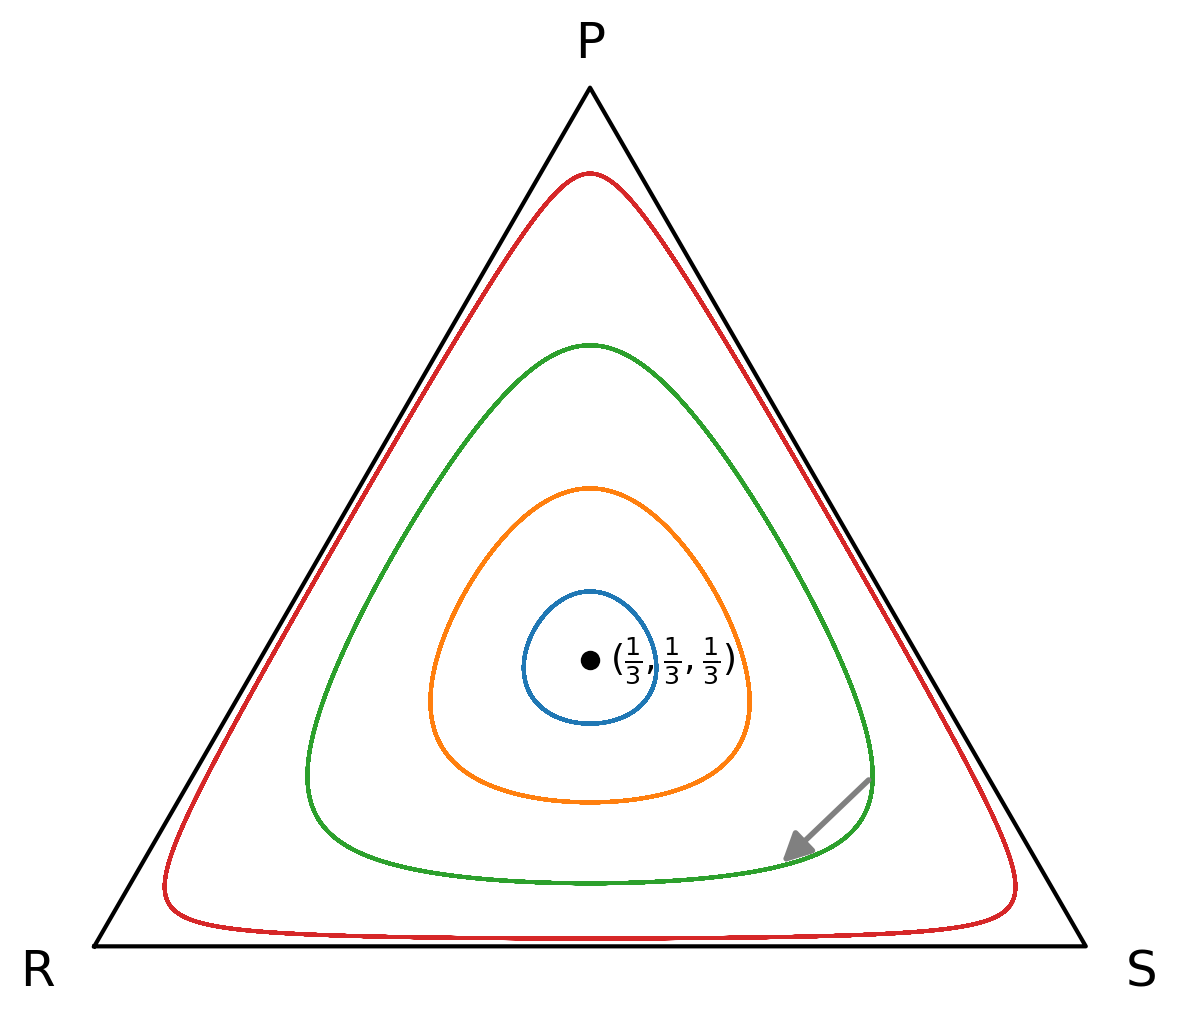
\includegraphics[width=0.5\textwidth]{figures/10_mathematical_ecology/rps-meanfield.png}
\label{fig:rps-replicator}
\end{center}
\end{figure}

% \clearpage

% \subsection*{Replicator dynamics and dominated strategies}

% \begin{itemize}
% \item A useful identity: for two strategies $i,j$ with $x_j > 0$,
% \[ \frac{\text{d}}{\text{d}t}\!\left[\frac{x_i}{x_j}\right] = \bigl[u(s_i,x) - u(s_j,x)\bigr]\, \frac{x_i}{x_j}. \]
% \item \textbf{Theorem.} If a pure strategy $s_i$ is strictly dominated (by some, possibly mixed, $y$), then for every interior initial condition $x_0$,
% \[ \lim_{t \to \infty} x_i(t) = 0. \]
% \item \emph{Sketch.} Set $v_i(x) = \log x_i - \sum_j y_j \log x_j$. Then
% \[ \frac{\text{d} v_i(x(t))}{\text{d} t} = \frac{\dot x_i}{x_i} - \sum_j y_j \frac{\dot x_j}{x_j} = u(s_i,x) - \sum_j y_j u(s_j,x) = u(s_i - y, x) < 0, \]
% since $s_i$ is strictly dominated by $y$. Hence $v_i(x(t)) \to -\infty$, so $x_i(t) \to 0$.
% \item \textbf{Theorem.} If $s_i$ is not rationalizable (i.e., is eliminated by iterated strict dominance), then $\lim_{t\to\infty} x_i(t) = 0$ for every interior $x_0$.
% \item \textbf{Reading:} replicator dynamics ``knows about'' dominance — it eventually purges dominated strategies, even without rational agents.
% \end{itemize}

% \subsection*{ESS and replicator dynamics}

\begin{itemize}
\item \textbf{Theorem.} Every ESS $x$ is an asymptotically stable steady state of the replicator dynamics. (If individuals can inherit mixed strategies, the converse is also true.)
% \item \textbf{Theorem.} If $x$ is an asymptotically stable steady state of the replicator dynamics, then $(x,x)$ is a perfect Nash equilibrium.
% \item Slogan: \emph{ESS} $\Longrightarrow$ \emph{asymptotic stability of replicator dynamics} $\Longrightarrow$ \emph{perfect Nash} $\Longrightarrow$ \emph{Nash}. The reverse implications can all fail (e.g.\ Rock--Scissors--Paper: Nash but no ESS, only neutral cycles).
\end{itemize}

So far, in a well-mixed population, defection wins. But people (and animals and institutions) often cooperate.\\
Why? The following mechanisms (from \hrefc{https://www.doi.org/10.1126/science.1133755}{Nowak, Science 2006}) each break the well-mixed assumption in a different way:
\begin{itemize}
\item repeated interactions (direct reciprocity);
\item reputation (indirect reciprocity);
\item networks / space;
\item in-group favoritism (theoretically, this does not work by itself!);
\item pay-it-forward / upstream reciprocity (theoretically, this does not work either!) — see the \hrefc{https://en.wikipedia.org/wiki/Pay_It_Forward_(film)}{2000 movie};
\item kin selection (J.\,B.\,S.\,Haldane: ``I would gladly give up my life for two brothers or eight cousins.'').
\end{itemize}

Real-world cooperation problems that need this theory: climate change, taxation, public spaces, sharing notes, group projects(!).

\subsection*{Direct reciprocity}

\subsubsection*{Tit-for-tat (TFT) and Axelrod's tournament}

\begin{itemize}
\item \hrefc{https://www.amazon.com/Evolution-Cooperation-Revised-Robert-Axelrod/dp/0465005640}{Axelrod (1984)} organized a computer tournament for the \emph{repeated} prisoner's dilemma. The next round of the game occurs with probability $w$ ($0 < w < 1$).
%
\pdmatrix{3}{0}{5}{1}
%
Example (C: cooperate, D: defect):
\begin{center}
\renewcommand{\arraystretch}{1.3}
\begin{tabular}{|l||c|c|c|c|c|c|c}
\hline
round & 1 & 2 & 3 & 4 & 5 & 6 & $\cdots$ \\
\hline\hline
A plays & C & D & D & C & D & C & $\cdots$ \\
\hline
B plays & C & C & D & C & D & D & $\cdots$ \\
\hline
A gets & 3 & 5 & 1 & 3 & 1 & 0 & $\cdots$ \\
\hline
\end{tabular}
\end{center}
A's accumulated payoff $= 3 + 5w + 1w^2 + 3w^3 + 1w^4 + 0w^5 + \cdots$.
%
\item \textbf{Question:} What is the maximum expected accumulated payoff a player can earn?
\item Why not just say e.g.\ $M=100$ games per pair?
\item Each algorithm played every other across many rounds; points $=$ payoff accumulated over rounds and opponents.
\item \textbf{Winner:} Tit-for-Tat (TFT), which cooperates on move 1 and then mimics the opponent's previous action. Very short, beats much more complicated algorithms.

\begin{verbatim}
IF n = 1:
    RETURN COOPERATE
ELSE:
    RETURN OpponentMove(n - 1)
\end{verbatim}

or

\begin{verbatim}
action = history[-1] if history else "COOPERATE"
\end{verbatim}

\item \textbf{Question:} Analyze TFT against
	\begin{itemize}
	\item ALLC (always cooperate),
	\item ALLD (always defect),
	\item TFT.
	\end{itemize}
Compute the accumulated payoff with discount factor $w$.
\item TFT works because it is
	\begin{itemize}
	\item \textbf{nice} (never defects first),
	\item \textbf{forgiving} (responds to a cooperation with cooperation),
	\item \textbf{retaliatory} (punishes defection immediately).
	\end{itemize}
\item Being only nice / only forgiving is not enough. Prof.\,\hrefc{https://fordschool.umich.edu/faculty/robert-axelrod}{Robert Axelrod} is here at U-M (Political Science \& Public Policy).
\end{itemize}

\subsubsection*{Under trembling hand: GTFT and WSLS}

\begin{itemize}
\item TFT is fragile to noise (``trembling hand'').
\item \textbf{Question:} Two TFT players. The first mistakenly defects in round 5. What happens after that? Compare payoffs to the error-free case.
\item Two strategies handle noise better than TFT:
	\begin{itemize}
	\item \textbf{Generous TFT (GTFT)}: like TFT, but also cooperate with small probability $q$ after the opponent defects.
		\begin{itemize}
		\item \textbf{Question:} In the setting above, suppose the second player is GTFT and forgives in round 10 (by playing C in round 10). What happens thereafter?
		\end{itemize}
	\item \textbf{Win-Stay--Lose-Shift (WSLS, ``Pavlov'')}: if the last round's outcome was $T$ or $R$, keep the same action; if it was $P$ or $S$, switch.
		\begin{itemize}
		\item Equivalent reading: ``satisfice'' — keep what you're doing if your payoff exceeds a threshold between $R$ and $P$. This is essentially \emph{reinforcement learning}.
		\item Unlike TFT and GTFT, WSLS depends on \emph{both} the opponent's and one's own last action.
		\end{itemize}
	\end{itemize}
\end{itemize}

\begin{itemize}
\item Satisficing with different aspiration levels (thresholds), with $T > R > P > S$. Strategy st$k$ keeps its action (green) if the reward is above its aspiration level (blue line) and switches its action (orange) otherwise.
\end{itemize}

\begin{center}
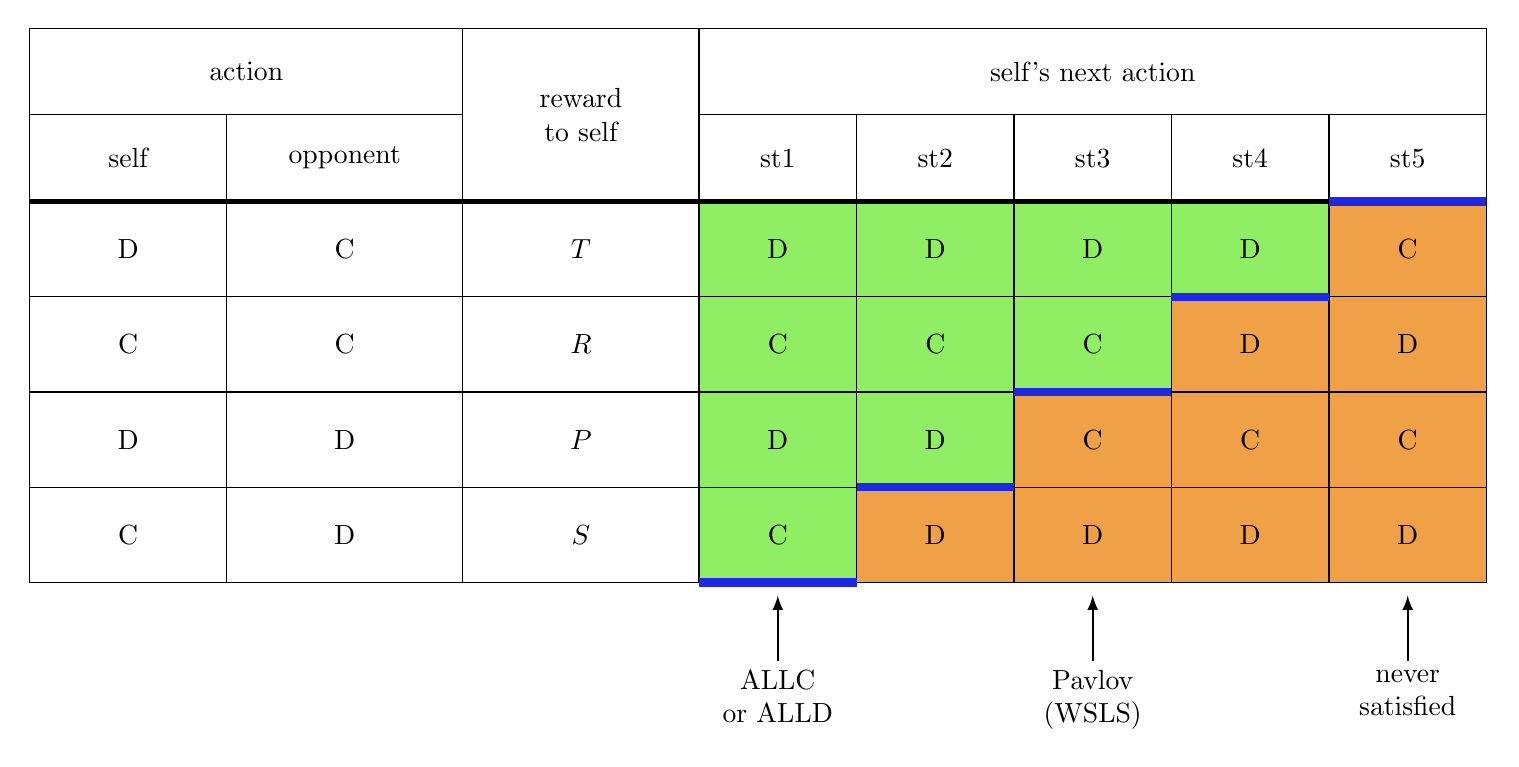
\begin{tikzpicture}[x=1.25cm,y=1.1cm]
\fill[stayc] (6.8,-2.00) rectangle (8.4,-3.10);
\node at (7.6,-2.55) {D};
\fill[stayc] (8.4,-2.00) rectangle (10.0,-3.10);
\node at (9.200000000000001,-2.55) {D};
\fill[stayc] (10.0,-2.00) rectangle (11.6,-3.10);
\node at (10.8,-2.55) {D};
\fill[stayc] (11.600000000000001,-2.00) rectangle (13.200000000000001,-3.10);
\node at (12.400000000000002,-2.55) {D};
\fill[shiftc] (13.2,-2.00) rectangle (14.799999999999999,-3.10);
\node at (14.0,-2.55) {C};
\node at (1,-2.55) {D}; \node at (3.2,-2.55) {C}; \node at (5.6,-2.55) {$T$};
\fill[stayc] (6.8,-3.10) rectangle (8.4,-4.20);
\node at (7.6,-3.65) {C};
\fill[stayc] (8.4,-3.10) rectangle (10.0,-4.20);
\node at (9.200000000000001,-3.65) {C};
\fill[stayc] (10.0,-3.10) rectangle (11.6,-4.20);
\node at (10.8,-3.65) {C};
\fill[shiftc] (11.600000000000001,-3.10) rectangle (13.200000000000001,-4.20);
\node at (12.400000000000002,-3.65) {D};
\fill[shiftc] (13.2,-3.10) rectangle (14.799999999999999,-4.20);
\node at (14.0,-3.65) {D};
\node at (1,-3.65) {C}; \node at (3.2,-3.65) {C}; \node at (5.6,-3.65) {$R$};
\fill[stayc] (6.8,-4.20) rectangle (8.4,-5.30);
\node at (7.6,-4.75) {D};
\fill[stayc] (8.4,-4.20) rectangle (10.0,-5.30);
\node at (9.200000000000001,-4.75) {D};
\fill[shiftc] (10.0,-4.20) rectangle (11.6,-5.30);
\node at (10.8,-4.75) {C};
\fill[shiftc] (11.600000000000001,-4.20) rectangle (13.200000000000001,-5.30);
\node at (12.400000000000002,-4.75) {C};
\fill[shiftc] (13.2,-4.20) rectangle (14.799999999999999,-5.30);
\node at (14.0,-4.75) {C};
\node at (1,-4.75) {D}; \node at (3.2,-4.75) {D}; \node at (5.6,-4.75) {$P$};
\fill[stayc] (6.8,-5.30) rectangle (8.4,-6.40);
\node at (7.6,-5.85) {C};
\fill[shiftc] (8.4,-5.30) rectangle (10.0,-6.40);
\node at (9.200000000000001,-5.85) {D};
\fill[shiftc] (10.0,-5.30) rectangle (11.6,-6.40);
\node at (10.8,-5.85) {D};
\fill[shiftc] (11.600000000000001,-5.30) rectangle (13.200000000000001,-6.40);
\node at (12.400000000000002,-5.85) {D};
\fill[shiftc] (13.2,-5.30) rectangle (14.799999999999999,-6.40);
\node at (14.0,-5.85) {D};
\node at (1,-5.85) {C}; \node at (3.2,-5.85) {D}; \node at (5.6,-5.85) {$S$};
\draw (0,0) rectangle (14.8,-6.40);
\draw (0,-1) -- (4.4,-1); \draw (6.8,-1) -- (14.8,-1);
\draw (0,-3.10) -- (14.8,-3.10);
\draw (0,-4.20) -- (14.8,-4.20);
\draw (0,-5.30) -- (14.8,-5.30);
\draw[line width=1.5pt] (0,-2) -- (14.8,-2);
\draw (2,-1) -- (2,-6.40); \draw (4.4,0) -- (4.4,-6.40); \draw (6.8,0) -- (6.8,-6.40);
\draw (8.4,-1) -- (8.4,-6.40);
\draw (10.0,-1) -- (10.0,-6.40);
\draw (11.600000000000001,-1) -- (11.600000000000001,-6.40);
\draw (13.2,-1) -- (13.2,-6.40);
\node at (2.2,-0.5) {action}; \node at (1,-1.5) {self}; \node at (3.2,-1.5) {opponent};
\node[align=center] at (5.6,-1) {reward\\to self};
\node at (10.8,-0.5) {self's next action};
\node at (7.6,-1.5) {st1};
\node at (9.2,-1.5) {st2};
\node at (10.8,-1.5) {st3};
\node at (12.4,-1.5) {st4};
\node at (14.0,-1.5) {st5};
\draw[threshc,line width=3pt] (6.8,-6.40) -- (8.4,-6.40);
\draw[threshc,line width=3pt] (8.4,-5.30) -- (10.0,-5.30);
\draw[threshc,line width=3pt] (10.0,-4.20) -- (11.600000000000001,-4.20);
\draw[threshc,line width=3pt] (11.600000000000001,-3.10) -- (13.2,-3.10);
\draw[threshc,line width=3pt] (13.2,-2.00) -- (14.8,-2.00);
\draw[-latex,thick] (7.6,-7.30) -- (7.6,-6.55);
\node[below,align=center] at (7.6,-7.30) {ALLC\\or ALLD};
\draw[-latex,thick] (10.8,-7.30) -- (10.8,-6.55);
\node[below,align=center] at (10.8,-7.30) {Pavlov\\(WSLS)};
\draw[-latex,thick] (14.0,-7.30) -- (14.0,-6.55);
\node[below,align=center] at (14.0,-7.30) {never\\satisfied};
\end{tikzpicture}

\textcolor{stayc!60!black}{green: win-stay (satisfice)};
\textcolor{shiftc!80!black}{orange: lose-shift};\\
\textcolor{threshc}{blue line: aspiration level (satisfaction threshold)}.
\end{center}

\begin{figure}[h]
\begin{center}
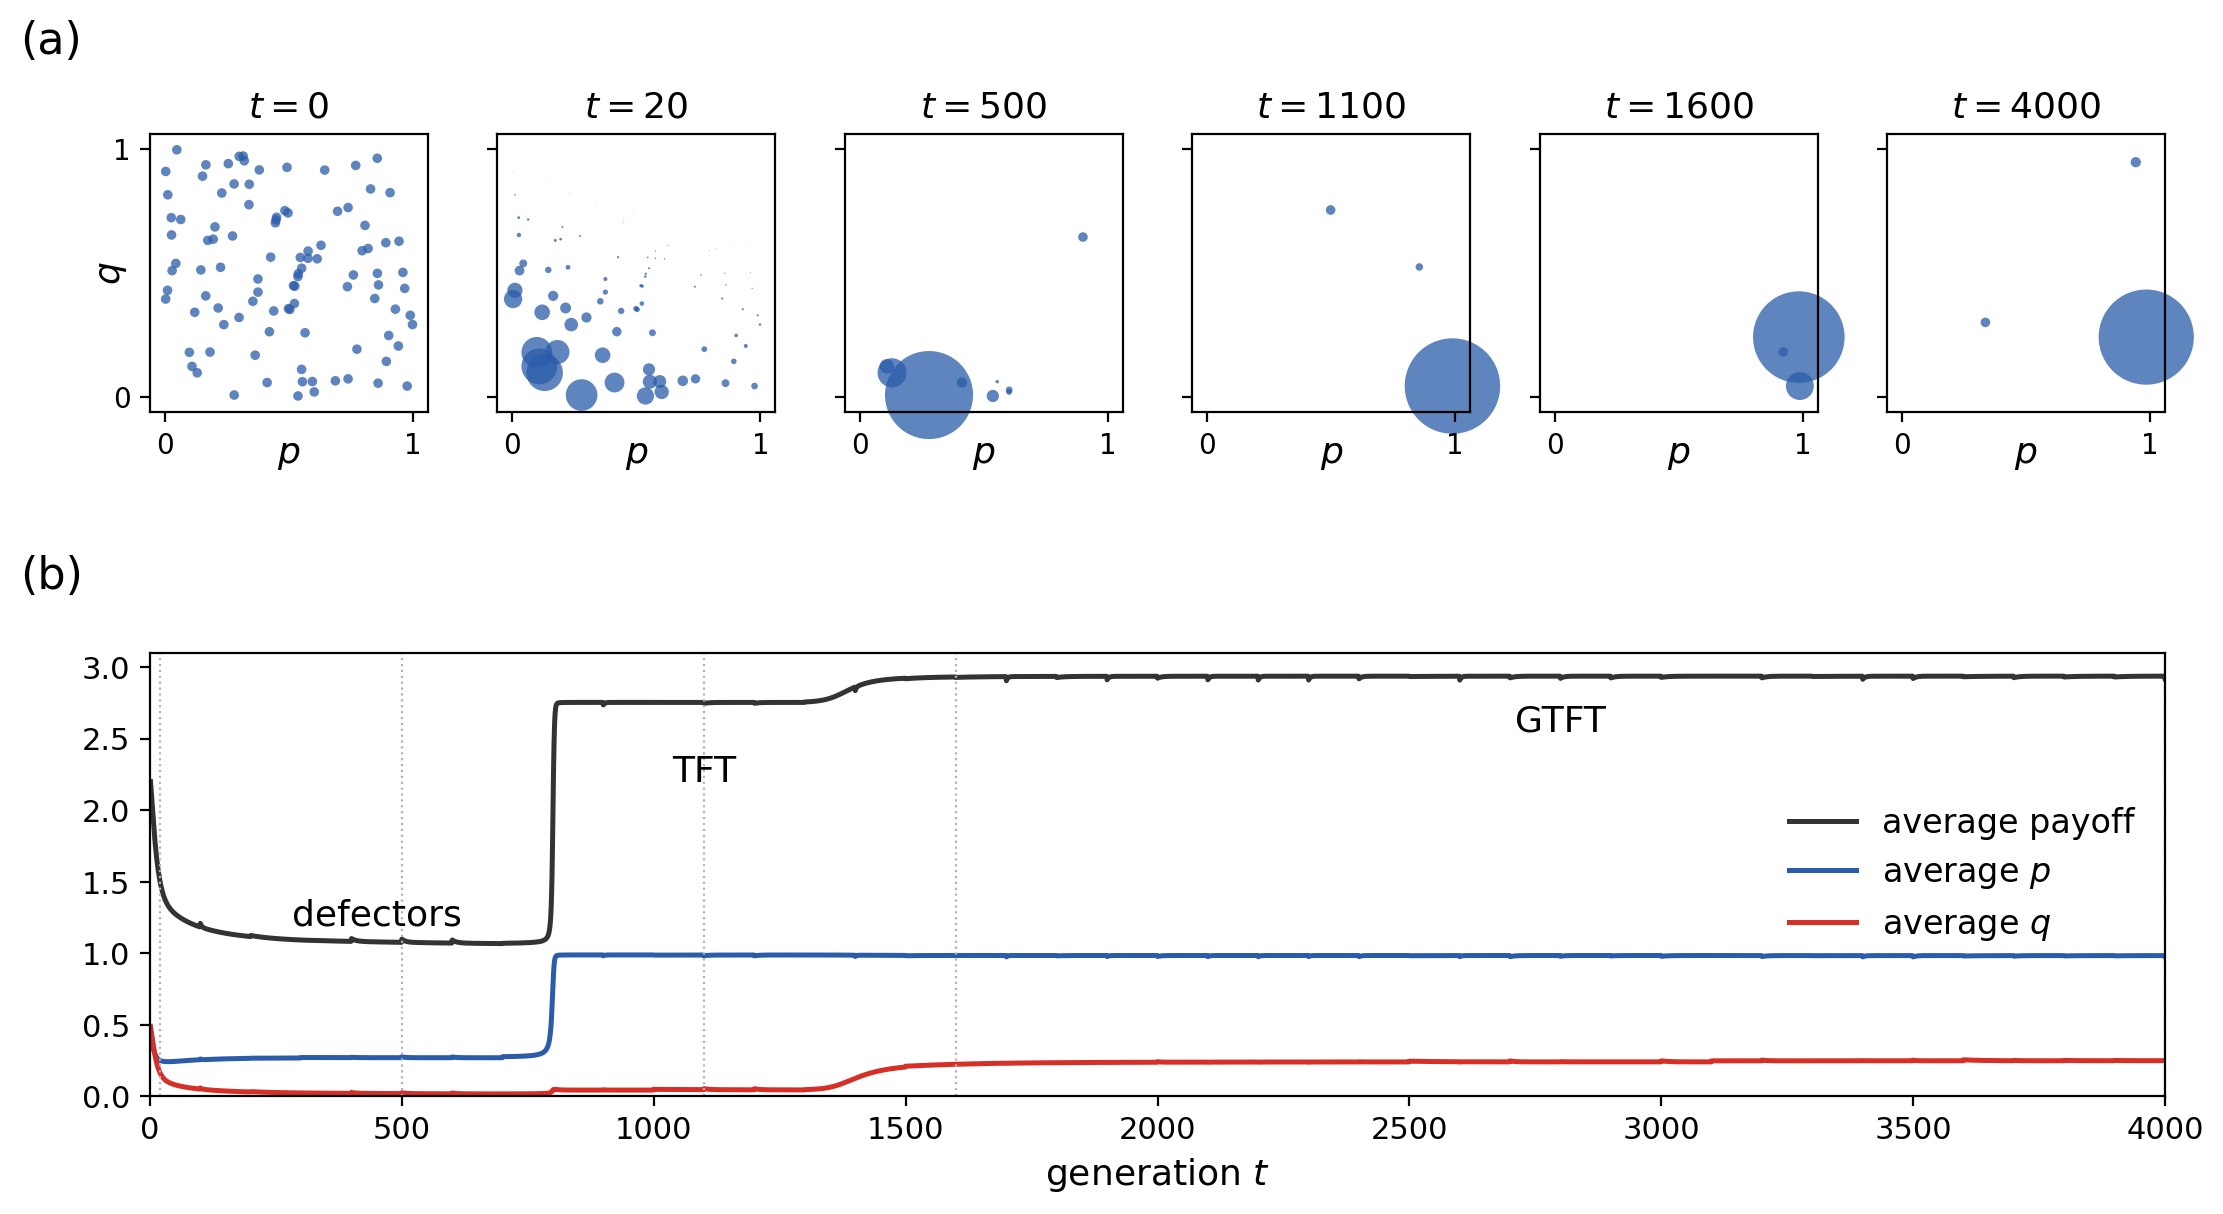
\includegraphics[width=\textwidth]{figures/11_evolutionary-games/reactive-gtft.png}
\caption{Evolution of GTFT. $p$ is the probability of cooperating right after the opponent cooperates; $q$ is the probability of cooperating right after the opponent defects. One run starting from 100 random strategies, with occasional mutants. (a) The population in the $(p,q)$ plane; disk area is proportional to frequency. (b) Population averages. Own simulation, after Fig.~1 of \hrefc{https://doi.org/10.1038/355250a0}{Nowak \& Sigmund, Nature (1992)}.}
\end{center}
\end{figure}

\begin{figure}[h]
\begin{center}
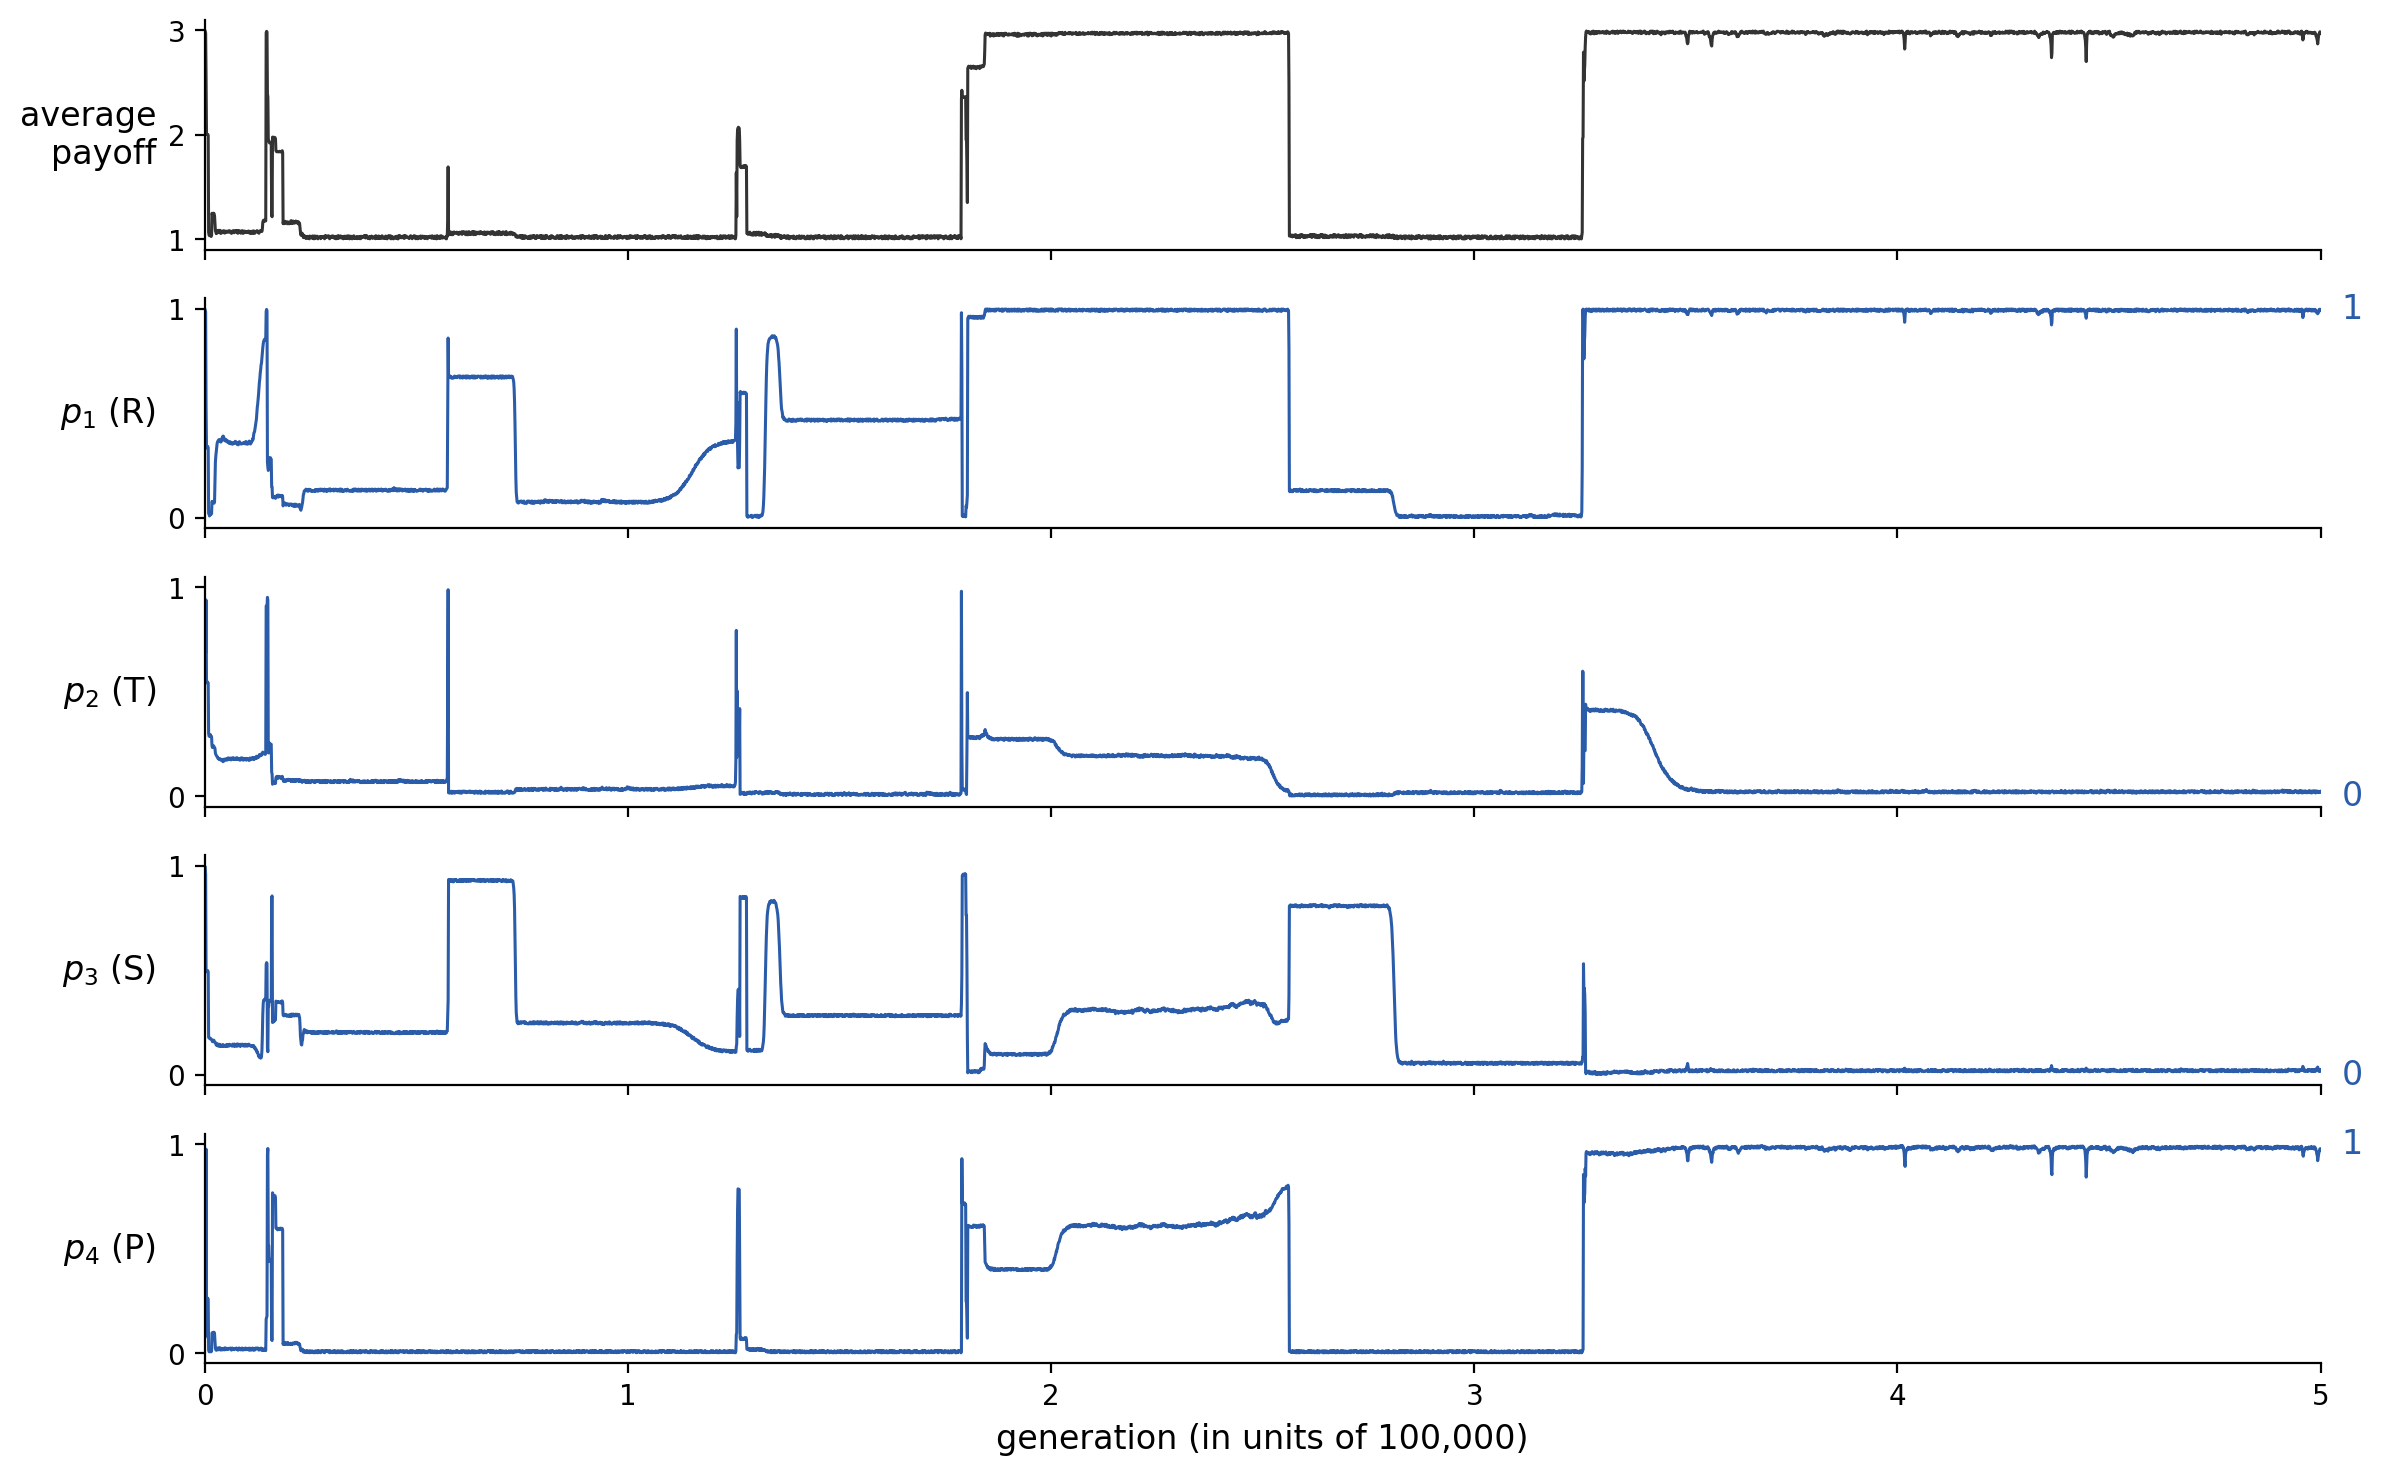
\includegraphics[width=\textwidth]{figures/11_evolutionary-games/memory-one-wsls.png}
\caption{Evolution of WSLS. $p_1, p_2, p_3, p_4$ are the probabilities of cooperating after $R$, $T$, $S$, $P$, respectively. One run with occasional mutants; the panels show population averages. WSLS $=(1,0,0,1)$ eventually takes over. Own simulation, after Fig.~1 of \hrefc{https://doi.org/10.1038/364056a0}{Nowak \& Sigmund, Nature (1993)}.}
\end{center}
\end{figure}

\subsection*{Spatial (and network) reciprocity}

\begin{figure}[h]
\begin{center}
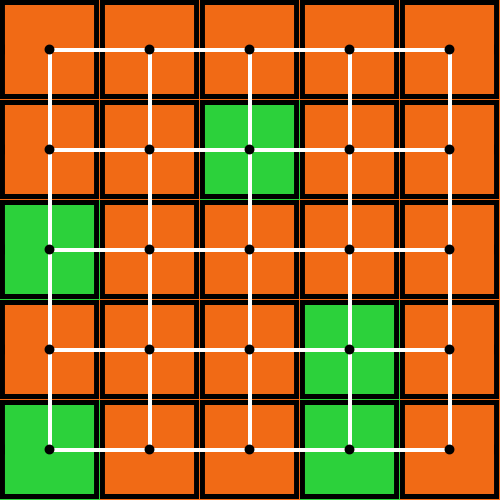
\includegraphics[width=0.4\textwidth]{figures/11_evolutionary-games/regular-network-vn-box-diff-strategies.png}
\caption{Interaction on a square lattice. Green: cooperator. Orange: defector. Figure~4(b) of chapter I-1 of \hrefc{https://wisc.pb.unizin.org/agent-based-evolutionary-game-dynamics/chapter/i-1/}{Izquierdo, Izquierdo \& Sandholm, Agent-Based Evolutionary Game Dynamics (2024)}, licensed under \hrefc{https://creativecommons.org/licenses/by/4.0/}{CC BY 4.0}.}
\end{center}
\end{figure}

\begin{itemize}
\item Each agent plays the prisoner's dilemma against all of its lattice neighbors and sums up the payoffs.

\pdmatrix{3}{0}{5}{1}

	\begin{itemize}
	\item \textbf{Question:} Compute the payoff of each agent on the above $5\times 5$ lattice (periodic boundary conditions).
	\end{itemize}
\item Each agent tends to mimic the strategy (C or D) of a successful neighbor in each generation.
	\begin{itemize}
	\item Social learning.
	\item Specify an imitation rule — details matter.
	\item If an agent is already more successful than all neighbors, it keeps its strategy.
	\end{itemize}
\item Run the ABM for a long time. Cooperators survive unless $T$ (temptation) is excessively large.
\item Cooperators form clusters that protect each other from exploitation by defectors.
	\begin{itemize}
	\item \textbf{Question:} Really? Consider a $5\times 5$ lattice with periodic boundary conditions. Place a $3 \times 3$ block of cooperators in the center; the remaining 16 cells are defectors. Compute the payoff of every player and check whether the clustering effect is visible.
	\item ``Make a good club of people.''
	\end{itemize}
\end{itemize}

\clearpage

\begin{figure}[h]
\begin{center}
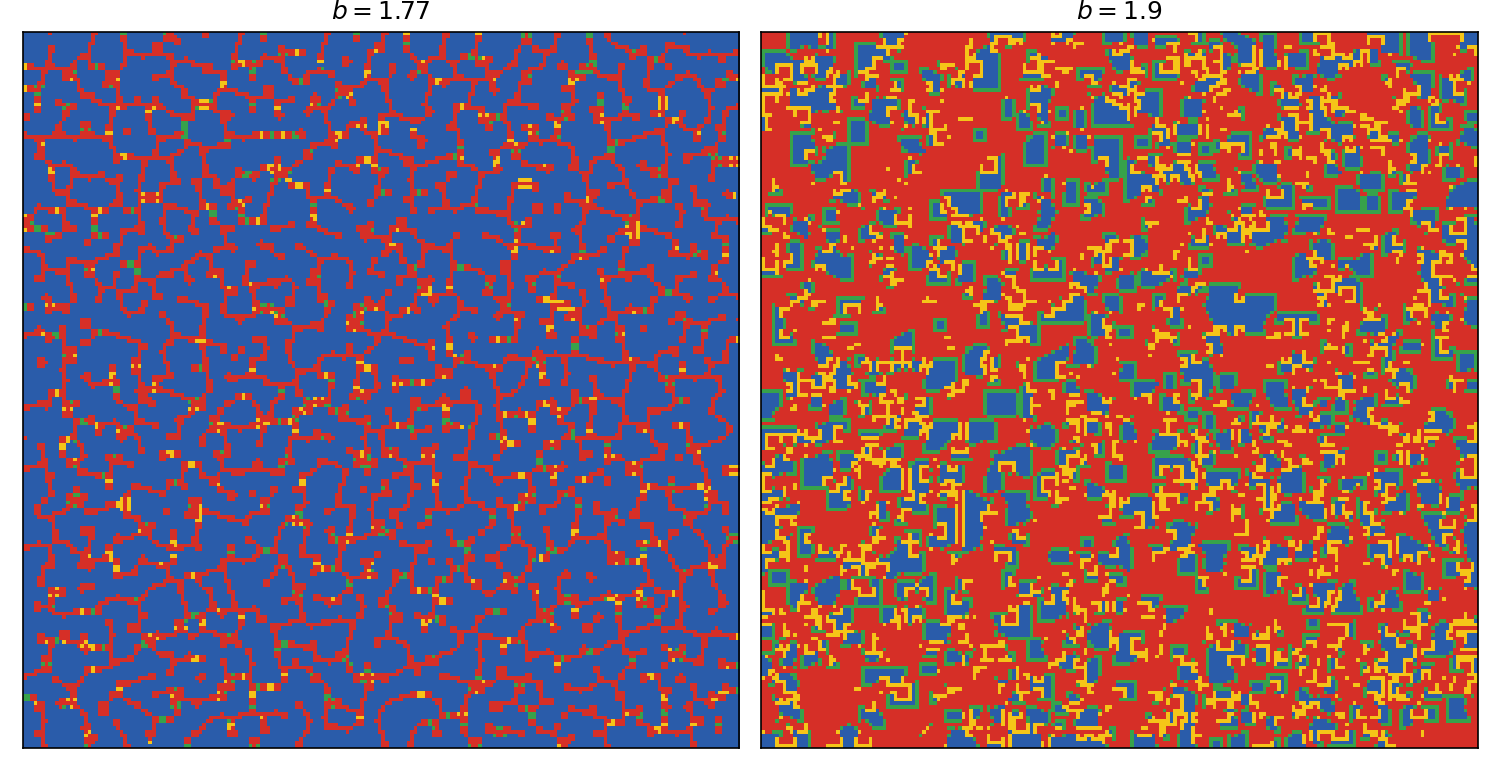
\includegraphics[width=0.75\textwidth]{figures/11_evolutionary-games/spatial-pd-random.png}\\[2mm]
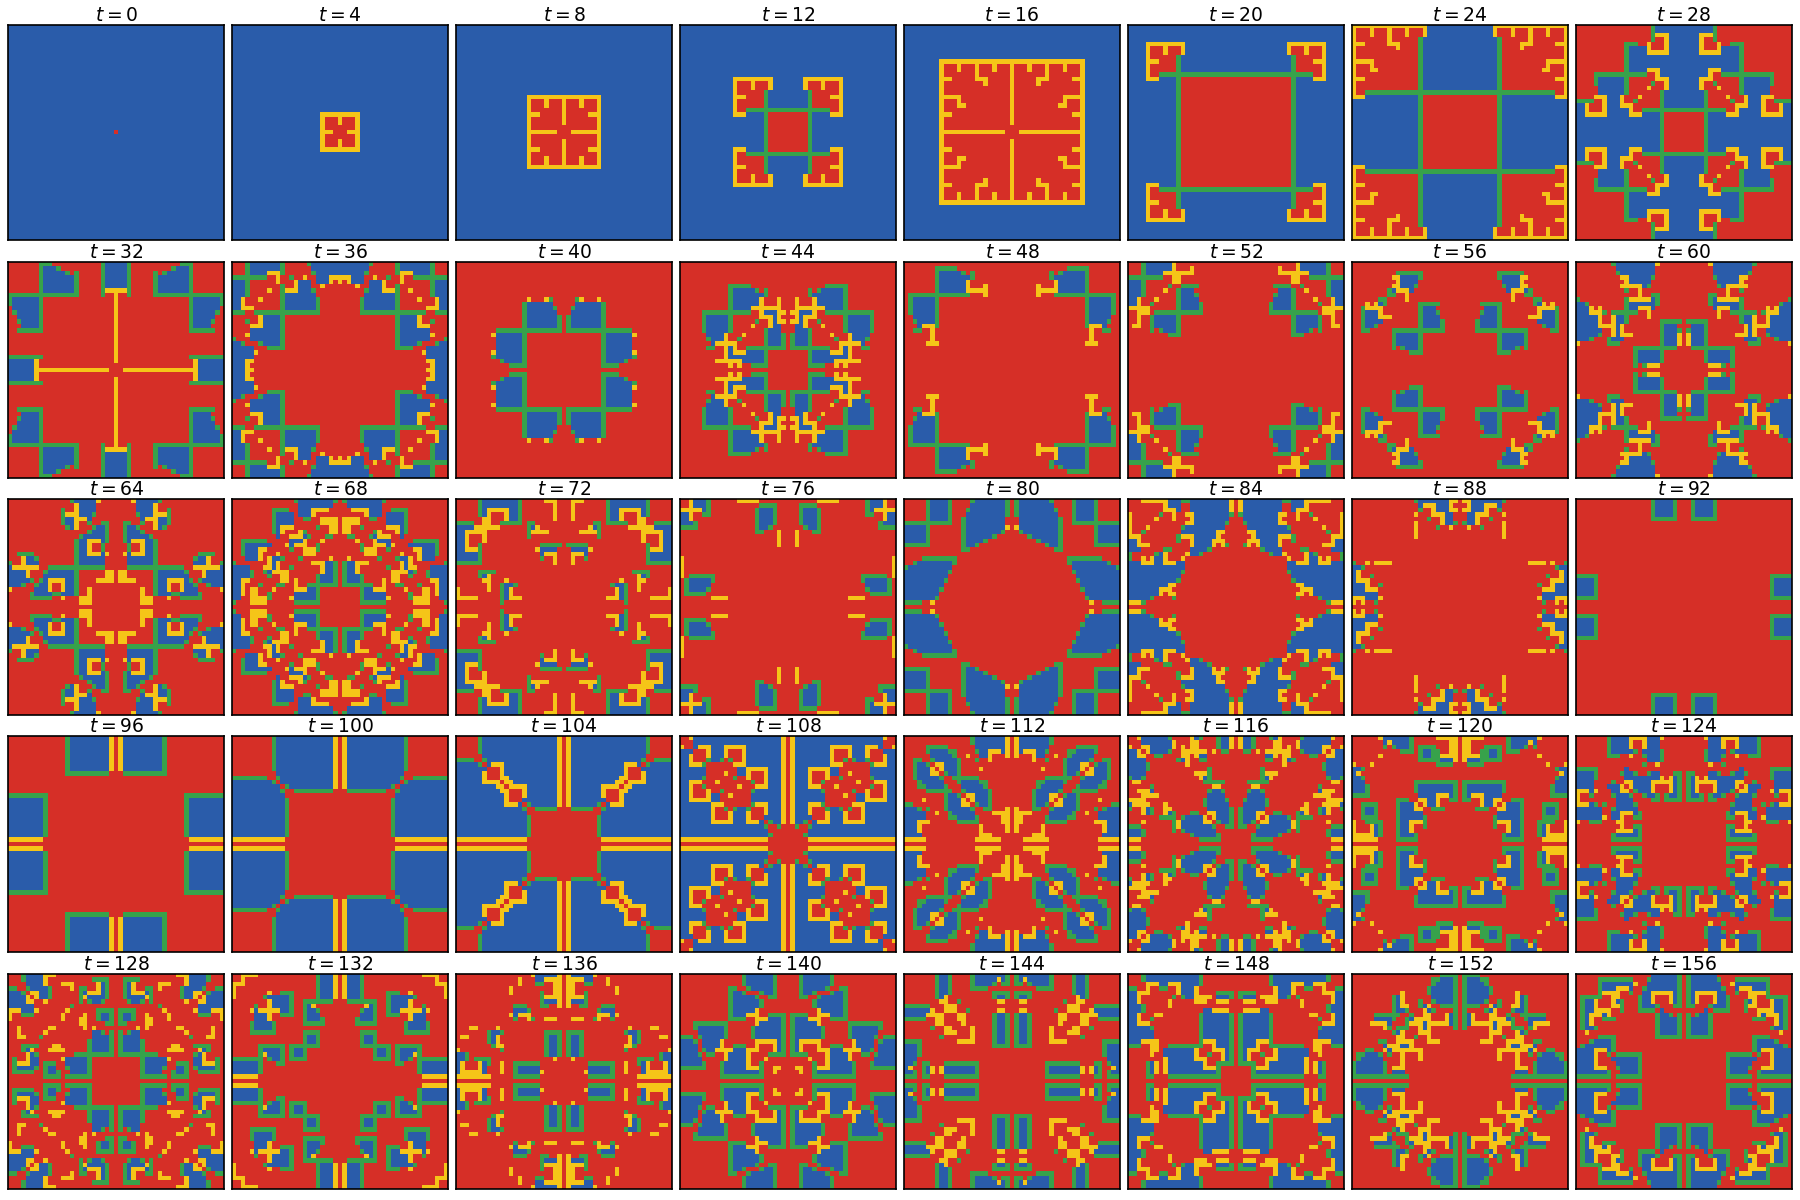
\includegraphics[width=0.75\textwidth]{figures/11_evolutionary-games/spatial-pd-kaleido.png}
\caption{Spatial reciprocity under a deterministic rule (more aesthetic than realistic), called spatial chaos. Blue: $C \to C$. Red: $D \to D$. Yellow: $C \to D$. Green: $D \to C$.
Top: 10\% defectors at random, after 200 generations. Bottom: a single defector invades cooperators ($b=1.85$).
Own simulations, after Fig.~1 of \hrefc{https://doi.org/10.1038/359826a0}{Nowak \& May, Nature (1992)} and Fig.~4 of \hrefc{https://doi.org/10.1142/S0218127493000040}{Nowak \& May, IJBC (1993)}.}
\end{center}
\end{figure}

\clearpage

\begin{figure}[h]
\begin{center}
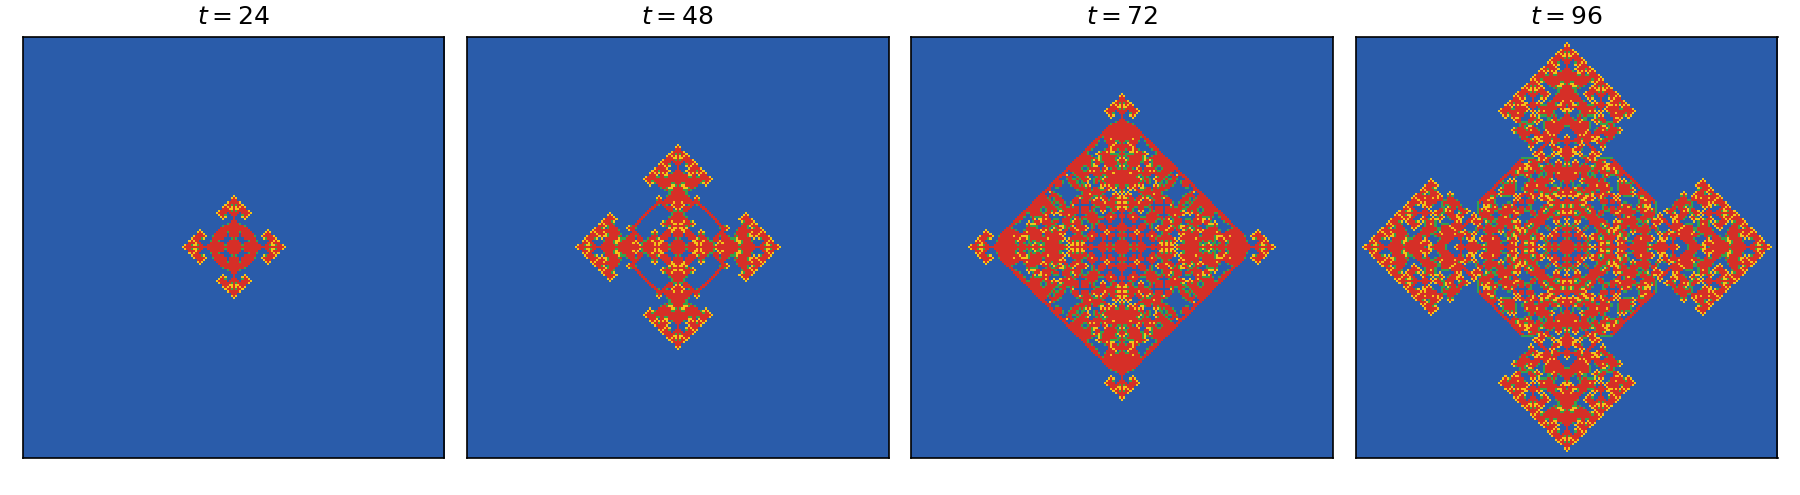
\includegraphics[width=\textwidth]{figures/11_evolutionary-games/spatial-pd-fractal.png}
\caption{A dynamic fractal: a single defector on an unbounded square lattice, with four neighbors per player ($b=1.8$). Own simulation, after Fig.~11 of \hrefc{https://doi.org/10.1142/S0218127493000040}{Nowak \& May, IJBC (1993)}.}
\end{center}
\end{figure}

\clearpage

\subsection*{Replicator equations with loners}

\begin{itemize}
\item Allow a third strategy, \emph{loners}, who do not participate in the public goods game.
\item Replicator dynamics give
\[
\begin{cases}
\dot{x} &= \ldots,\\
\dot{y} &= \ldots,\\
\dot{z} &= \ldots,
\end{cases}
\]
with $x+y+z=1$. Dynamics live on the 2-simplex.
\item Result: cooperation is maintained through rock--scissors--paper-style cycling among cooperators, defectors, and loners.
\end{itemize}

\begin{figure}[h]
\begin{center}
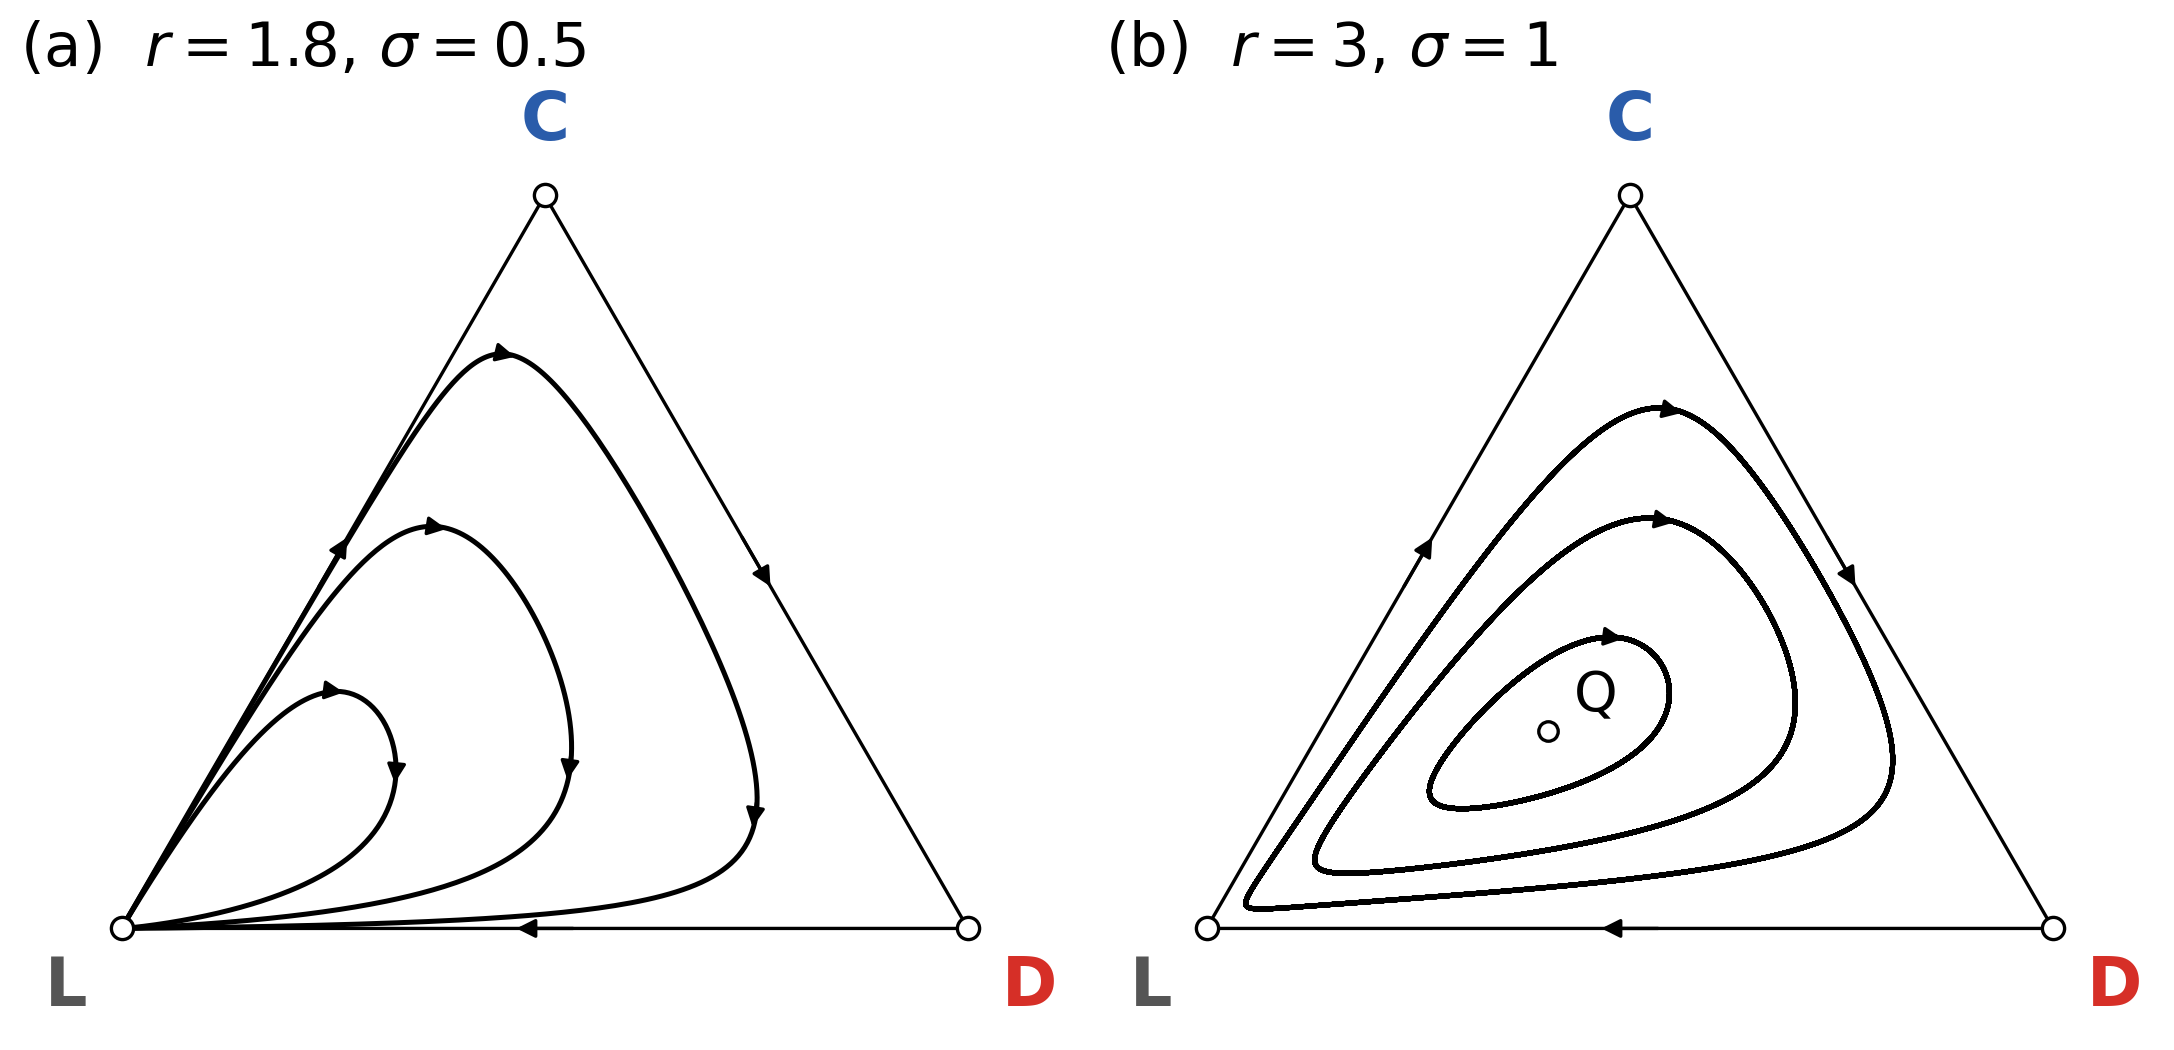
\includegraphics[width=0.65\textwidth]{figures/11_evolutionary-games/loners-replicator.png}
\caption{Replicator dynamics of the public goods game with loners ($N=5$). (a) $r<2$: cooperation does not emerge. (b) $r>2$: cooperation persists through cycles of cooperators (C), defectors (D), and loners (L) around the fixed point $Q$. Own simulation, after Fig.~1(A, B) of \hrefc{https://www.doi.org/10.1126/science.1070582}{Hauert et al., Science (2002)}.}
\end{center}
\end{figure}

\clearpage

\subsection*{Vaccination dilemma}

\begin{itemize}
\item Voluntary vaccination is a public-goods dilemma. When I vaccinate,
	\begin{itemize}
	\item I pay a cost (money, time, side-effect risk).
	\item I also add to \emph{herd immunity}, which protects everyone, including those who do not vaccinate.
	\end{itemize}
\item So there is a temptation to \emph{free-ride}: skip vaccination and rely on others' vaccination to avoid infection.
	\begin{itemize}
	\item This is a prisoner's dilemma / public-goods game situation.
	\item \textbf{Q:} self-interested equilibrium? 
	% gives \emph{less} vaccination than the social optimum.
	\end{itemize}
\item When uptake is voluntary, coverage can fall below the level needed for herd immunity.
	\begin{itemize}
	\item E.g., the sharp drop in MMR vaccination in Britain after a vaccine--autism scare.
	\item COVID-19?
	\end{itemize}
\item \hrefc{https://doi.org/10.1098/rspb.2010.1107}{Fu, et al., Proc.\ R.\ Soc.\ B (2011)} study this with \emph{evolutionary game theory}.
	\begin{itemize}
	\item Instead of perfectly rational agents, people imitate peers who seem to be doing well.
	\end{itemize}
\end{itemize}

\subsubsection*{Model: a two-stage seasonal game}

\begin{itemize}
\item Each season has two stages:
	\begin{enumerate}
	\item \textbf{Vaccination choice.} A fraction $x$ of the population vaccinates. Vaccination costs $V$ and gives perfect immunity.
	\item \textbf{Epidemic (health outcome).} The disease spreads among the unvaccinated by the SIR model. An unvaccinated person who gets infected pays a cost $I$.
	\end{enumerate}
%
\begin{figure}[h]
\begin{center}
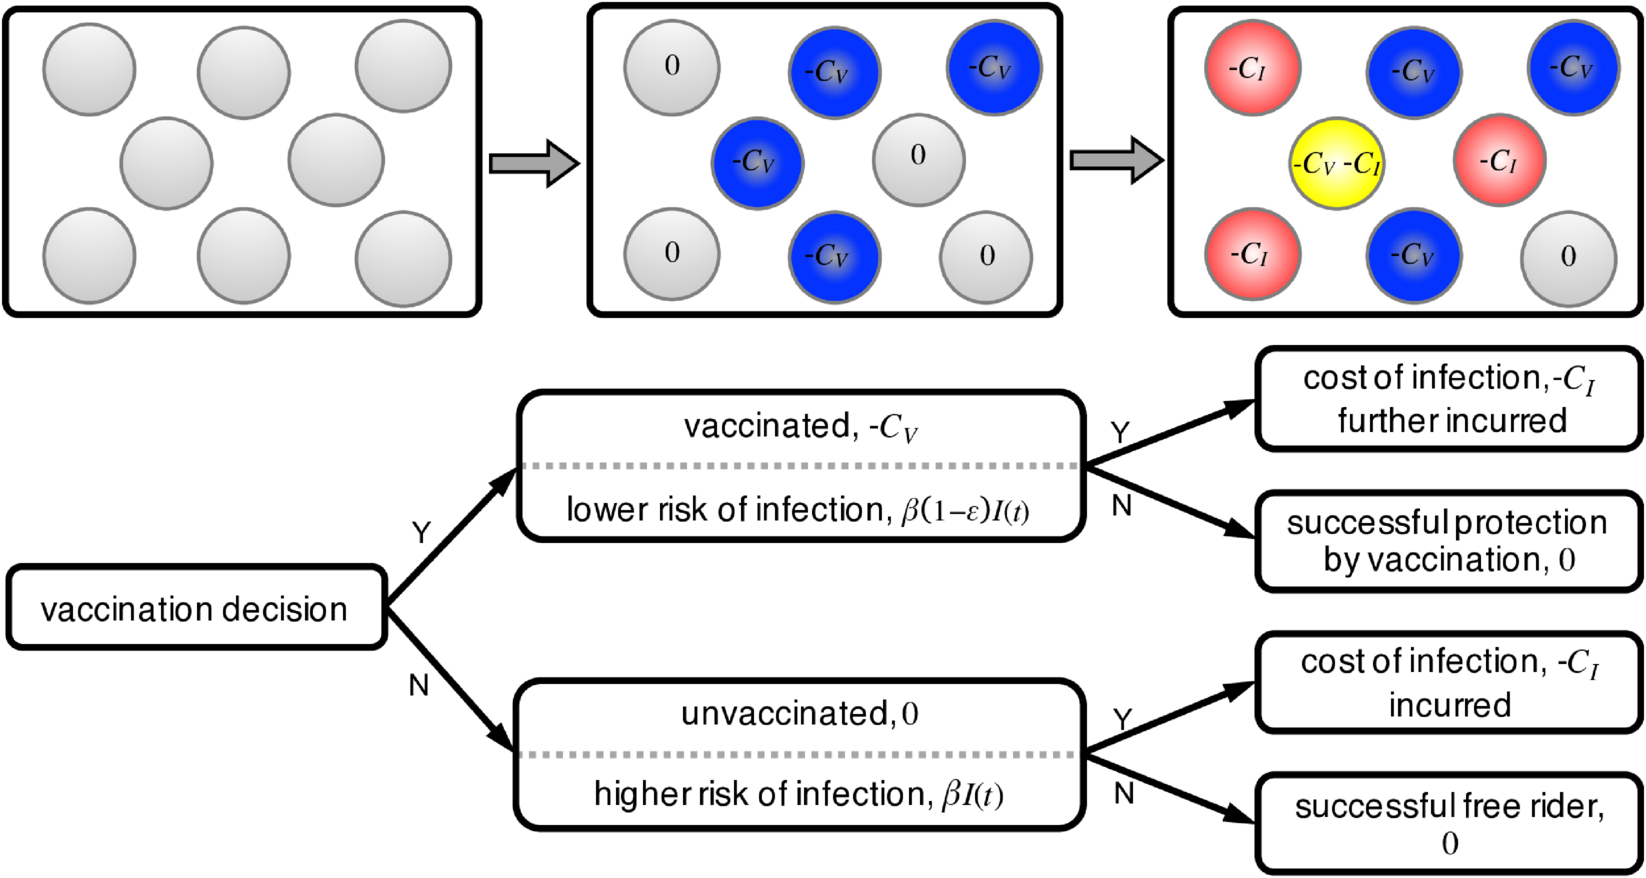
\includegraphics[width=0.8\textwidth]{figures/11_evolutionary-games/Fu2025-schematic.png}
\caption{The two-stage vaccination game. $C_V$ and $C_I$ correspond to our $V$ and $I$. This figure allows an imperfect vaccine with efficacy $\varepsilon$; our model assumes $\varepsilon = 1$. Figure~1 of \hrefc{https://doi.org/10.1371/journal.pcbi.1013586}{Fu, Zhuo \& Chen, PLOS Computational Biology (2025)}, licensed under \hrefc{https://creativecommons.org/licenses/by/4.0/}{CC BY 4.0}.}
\label{fig:fu-schematic}
\end{center}
\end{figure}
%
\item Payoffs at the end of a season:
\[
\begin{aligned}
\text{vaccinated} &: -V,\\
\text{unvaccinated \& infected} &: -I,\\
\text{unvaccinated \& healthy} &: 0.
\end{aligned}
\]
\item The ``unvaccinated \& healthy'' individuals are the successful free-riders (highest payoff, $0$). 
\item Only the ratio matters, so define the relative cost of vaccination by $c = V/I \in (0,1)$.
\item Stage 2 (epidemic): With basic reproduction number $R_0$ and a fraction $x$ vaccinated, the SIR \emph{final-size} relation gives the infection risk of an unvaccinated individual,
\[ \frac{R(\infty)}{1-x} = 1 - e^{-R_0 R(\infty)}, \]
where $R(\infty)$ is the fraction ever infected. Vaccinating a fraction above the \emph{herd-immunity threshold}
\[ x_{\rm c} = 1 - \frac{1}{R_0} \]
drives the epidemic to (almost) zero.
\item After each season, each individual $i$ picks a random role model $j$ and copies $j$'s strategy (vaccinate or not) with probability given by the \emph{Fermi function}
\[ f(P_j - P_i) = \frac{1}{1 + \exp[-\beta (P_j - P_i)]}. \]
	\begin{itemize}
	\item $P_i, P_j:$ payoffs,
	\item $\beta>0$ is the \emph{selection strength} (how strongly people favour higher-payoff strategies).
		\begin{itemize}
		\item \textbf{Q:} What happens in the limit $\beta\to\infty$?
		\item \textbf{Q:} How about $\beta = 0$?
		\item To first order in $\beta$, reduces to the replicator dynamics. \textbf{Q:} How to show that?
		\item Who is Fermi?
		\end{itemize}
	\end{itemize}
\end{itemize}

Results:
\begin{itemize}
\item Vaccination decreases and the final epidemic size increases as $c$ increases.
\item Paradox: For strong selection ($\beta = 10$), i.e., when people imitate apparent winners more aggressively, the equilibrium vaccination level drops (further), and the epidemic is correspondingly larger.
	\begin{itemize}
	\item Being better at copying successful peers makes the population worse off, because the most ``successful'' peers are the lucky free-riders.
	\end{itemize}
\item In structured populations (lattices / random networks; not shown here), vaccination stays high for low cost $c$ but collapses abruptly once $c$ passes a threshold.
	\begin{itemize}
	\item Echoing historical episodes where coverage held for years and then dropped sharply.
	\end{itemize}
\item No free lunch.
\item Take-home: Coupling a game with an epidemic. Application of evolutionary game theory (essentially, imitation dynamics) for human behavior to a public-health problem.
\end{itemize}

\subsection*{Cancer as an evolutionary game}

\subsubsection*{Motivation}

\begin{itemize}
\item A tumor is not a uniform clone: it is a genetically heterogeneous population of cells that mutate, compete for space and resources, and are selected.
	\begin{itemize}
	\item Darwinian evolution inside the body.
	\item A cell's ``payoff'' $=$ its proliferative \emph{fitness}.
	\end{itemize}
\begin{figure}[h]
\begin{center}

\includegraphics[width=0.35\textwidth]{figures/11_evolutionary-games/Commons-calico-cat.jpg}
\caption{Name? Why am I showing this? \hrefc{https://commons.wikimedia.org/wiki/File:Calico_Cat_in_2024_2.jpg}{``Calico Cat in 2024 2''} by Vitorperrut555, Wikimedia Commons, released into the public domain under \hrefc{https://creativecommons.org/publicdomain/zero/1.0/}{CC0 1.0}.}
\label{fig:calico}
\end{center}
\end{figure}
\item Why a game (frequency-dependent), and not just constant selection? Many cancer cells secrete diffusible growth factors that also help neighboring cells --- a public good. A cell's fitness then depends on what its neighbors do, which is exactly the frequency-dependent setting of evolutionary game theory.
	\begin{itemize}
	\item Cooperation among cancer cells cannot be explained as ``for the good of the tumour''.
		\begin{itemize}
		\item A mutant that stops producing the growth factor still enjoys the factor made by others, so it \emph{free-rides} and spreads.
		\item A tragedy of the commons at the cellular level (cf.\ the prisoner's dilemma / public-goods game earlier).
		\end{itemize}
	\end{itemize}
\item Authority review: \hrefc{https://doi.org/10.1038/s41568-018-0083-7}{Archetti \& Pienta, Nature Reviews Cancer (2019)}. (The idea goes back to \hrefc{https://doi.org/10.1016/S0959-8049(97)00170-6}{Tomlinson, Eur.\ J.\ Cancer (1997)}.)
\end{itemize}

\subsubsection*{Cancer cells play a public-goods game}

\begin{itemize}
\item Two cell types:
	\begin{itemize}
	\item Producers (cooperators), which secrete the growth factor at a cost $c$,
	\item Non-producers (free-riders), which do not.
	\end{itemize}
\item If the benefit of the growth factor were linear in its amount, free-riders would always win and producers would vanish (a prisoner's dilemma).
\item But, growth-factor benefit is typically nonlinear (saturating/sigmoidal in concentration), turning it into a snowdrift-/Chicken-like or threshold public-goods game (cf.\ the Hawk--Dove and public-goods).
\item Outcome:
	\begin{itemize}
	\item If the cost-to-benefit ratio $c$ is high, non-producers have higher fitness at every frequency, so producers are eliminated.
	\item If $c$ is low enough, producers have the advantage when rare, and the population settles at a stable mixed equilibrium of producers and free-riders.
	\end{itemize}
\item This explains a hallmark of tumors: persistent \emph{intratumor heterogeneity} (coexistence of distinct cell types).
	\begin{itemize}
	\item Analogous to a mixed ESS.
	\end{itemize}
\item As with public goods generally, the equilibrium is \emph{inefficient}, i.e., fewer producers than would maximize total tumor growth.
\end{itemize}

\begin{figure}[h]
\begin{center}
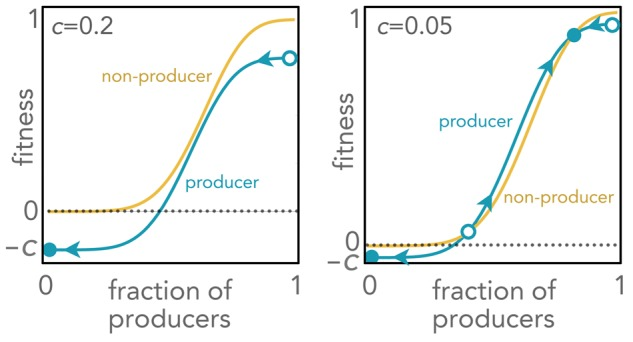
\includegraphics[width=0.6\textwidth]{figures/11_evolutionary-games/Archetti2018-game.png}
\caption{Cancer cells as a public-goods game. Left: high cost. Right: low cost. Filled circles: stable equilibria. Open circles: unstable equilibria. Figure~2 of \hrefc{https://doi.org/10.1093/emph/eoy003}{Archetti, Evolution, Medicine, and Public Health (2018)}, licensed under \hrefc{https://creativecommons.org/licenses/by/4.0/}{CC BY 4.0}.}
\label{fig:cancer-game}
\end{center}
\end{figure}

\clearpage

\subsubsection*{Adaptive therapy}

\begin{itemize}
\item The game viewpoint changes how we should \emph{treat} cancer.
\item Standard chemotherapy gives the maximum tolerated dose (MTD).
	\begin{itemize}
	\item Kills drug-sensitive cells.
	\item But \emph{selects for} drug-resistant cells.
	\item Once the sensitive cells are gone, the resistant cells expand unchecked (``competitive release''), and the tumor relapses (\hrefc{https://doi.org/10.1158/0008-5472.CAN-08-3658}{Gatenby et al., Cancer Research (2009)}).
	\end{itemize}
\item Key idea: resistance carries a cost (resistant cells grow more slowly when the drug is absent). So a residual population of sensitive cells \emph{suppresses} the resistant cells through competition.
\item A minimal Lotka--Volterra model:
\[
\begin{aligned}
\frac{\text{d}S}{\text{d}t} &= r_S\, S\left(1 - \frac{S + R}{K}\right) - d(t)\, S,\\
\frac{\text{d}R}{\text{d}t} &= r_R\, R\left(1 - \frac{S + R}{K}\right).
\end{aligned}
\]
\begin{itemize}
\item $S$: density of sensitive cells,
\item $R$: density of resistant cells,
\item $r_R < r_S$ (cost of resistance),
\item $d(t)$: the drug-induced death of sensitive cells.
\end{itemize}
Under continuous MTD ($d$ large), $S\to0$ and then $R\to K$ (competitive release).
\item Adaptive therapy: treat only enough to contain the tumor, then pause.
\item Then, sensitive cells rebound and out-compete resistant cells, ``steering'' the tumor back to a treatable composition.
\item Repeat these steps.
\begin{figure}[h]
\begin{center}
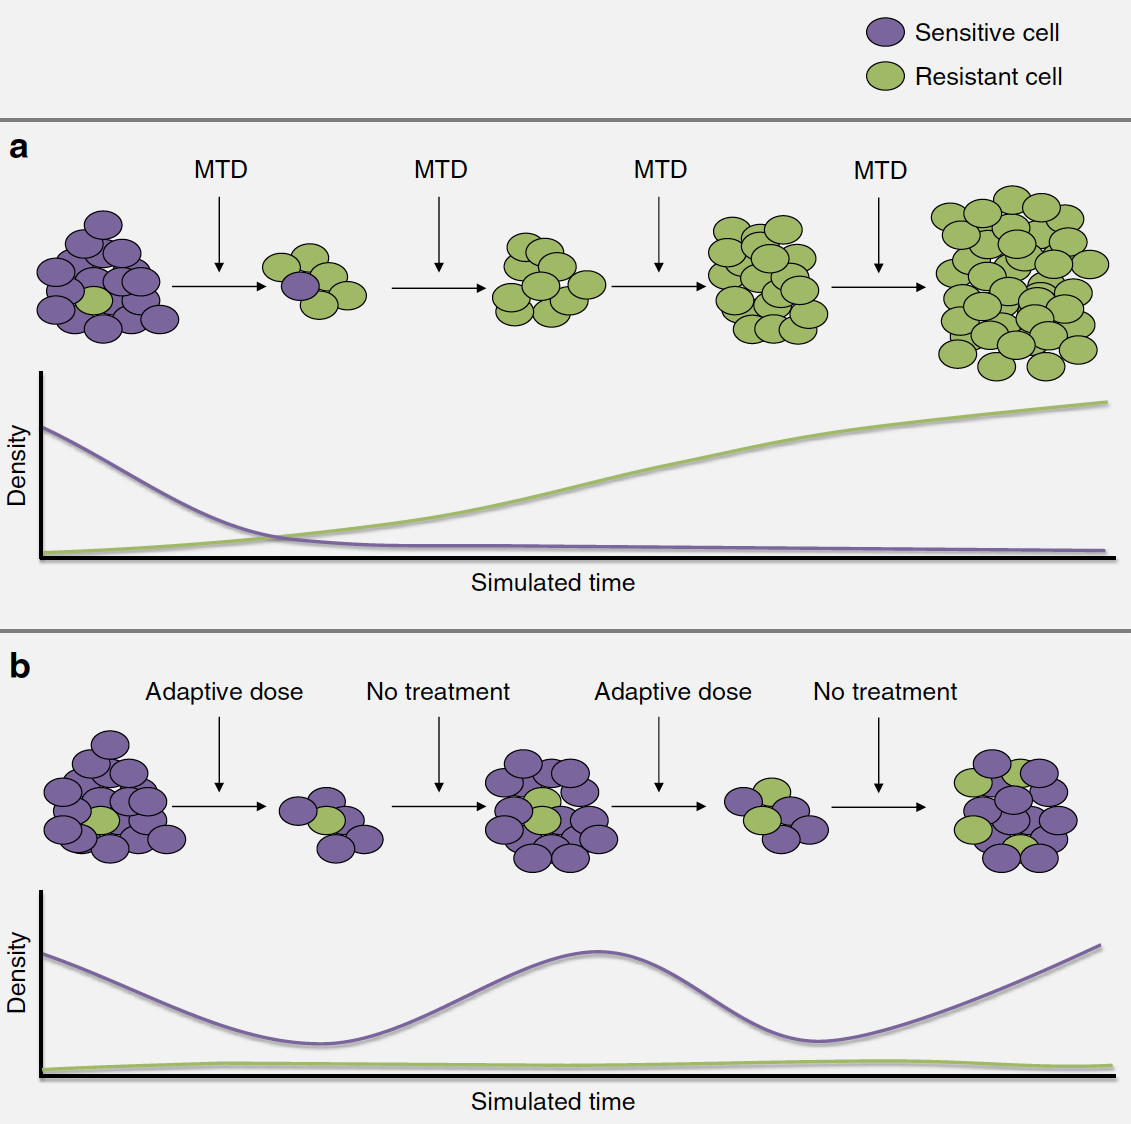
\includegraphics[width=0.85\textwidth]{figures/11_evolutionary-games/Zhang2017-adaptive.png}
\caption{(b) contains the tumor over many cycles. Figure~1 of \hrefc{https://doi.org/10.1038/s41467-017-01968-5}{Zhang et al., Nature Communications (2017)}, licensed under \hrefc{https://creativecommons.org/licenses/by/4.0/}{CC BY 4.0}.}
\label{fig:adaptive}
\end{center}
\end{figure}
\clearpage
\item Pilot clinical trial (\hrefc{https://doi.org/10.1038/s41467-017-01968-5}{Zhang, Cunningham, Brown \& Gatenby, Nature Communications (2017)})
	\begin{itemize}
	\item Metastatic castration-resistant prostate cancer treated with abiraterone.
	\item Cell populations were modeled by a Lotka--Volterra model with three subtypes (androgen-dependent, androgen-producing, and androgen-independent/resistant).
	\item Adaptive dosing kept 10 of 11 patients in stable tumor-burden oscillations, with median time to progression $\ge 27$ months (vs.\ $\sim$16.5 months under standard dosing) using roughly half the cumulative drug.
	\end{itemize}
\end{itemize}

\end{document}
